\section{Combination}	
\label{sec:bsintro} 
Here we detail the combination of the signal cross section upper limit sensitivity for the semileptonic, all-hadronic, and dileptonic $\bs$ decay channels.  
The specifics for the three searches are detailed in the analysis notes \cite{CMS-AN-14-049,CMS-AN-14-103,CMS-AN-13-415}.  Identical sources of systematic uncertainty are 
correlated across the channels.  The overlap of the signal region events is negligible.  There is no overlap between the all-hadronic channel and the other selections.  
The dileptonic channel and semileptonic have four overlapping events out of 7900 lepton+jets events and 17559 dilepton events.
and we set limits using the Bayesian statistical method as implemented by the theta 
framework to set 95\%C.L. upper limits on the $\bs \to \mathrm{tW}$ cross-section.

The following systematic uncertainties are correlated across multiple channels (see Section\ref{sec:bssystematics}):
	
\begin{itemize}
\item \textbf{Jet Energy Scale}
\item \textbf{Jet Energy Resolution}
\item \textbf{Luminosity}
\item \textbf{DiBoson Cross-Section}:  The semileptonic and dileptonic channels use the recommended 30\% uncertainty on the di-boson cross-section.  The all-hadronic channel does not 
include this background source.
\item \textbf{Single-top Cross-Section}
\item \textbf{Z+jets Cross-Section}:  The semileptonic and dileptonic channels use the recommended 20\% uncertainty on the Z+jets cross-section.  The all-hadronic channel does not 
include this background source.
\item \textbf{$\ttbar$ Cross-Section}:  The semileptonic and dileptonic channels use the recommended 5.3\% uncertainty on the $\ttbar$ cross-section.  The all-hadronic channel does not 
include this uncertainty due to a measurement of the $\ttbar$ normalization and uncertainty in the analysis.
\end{itemize}

Statistical uncertainties are taken into account by using the Barlow-Beeston lite method.

The rate effects of the systematic uncertainties that only affect the semileptonic channel are given in tables \ref{table:bsRsysSl1} and \ref{table:bsRsysSl2}  for the electron and muon channels respectively.
The rate effects of the systematic uncertainties that only affect the all-hadronic channel are given in table \ref{table:bsRsysHa}.
The rate effects of the systematic uncertainties that only affect the dileptonic channel are given in table \ref{table:bsRsysDi}.
The rate effects of the systematic uncertainties that are correlated over multiple channels are given in table \ref{table:bsRsysCoSe}, \ref{table:bsRsysCoSm}, 
\ref{table:bsRsysCoH}, \ref{table:bsRsysCoD} for the semileptonic electron, semileptonic muon, all hadronic, and dilepton channels respectively.

The nuisance parameters after the Theta fit can be seen in figure \ref{figs:bsnuisance}.

The distributions given to the limit setting macro are shown in figures \ref{figs:bsmtwsemi}, \ref{figs:bsmtwdilep}, and \ref{figs:bsmtwallhad} for the semileptonic, dileptonic, and all-hadronic 
channels respectively.  The limits for the three channels before combination are shown in figure \ref{figs:bslimitssemi}, \ref{figs:bslimitsdilep}, and \ref{figs:bslimitshad}  for the semileptonic, dileptonic, and all-hadronic 
channels respectively.  The combined limits are shown in Figure \ref{figs:bsthetalimit}.  


\begin{figure}[htcb]
\centering
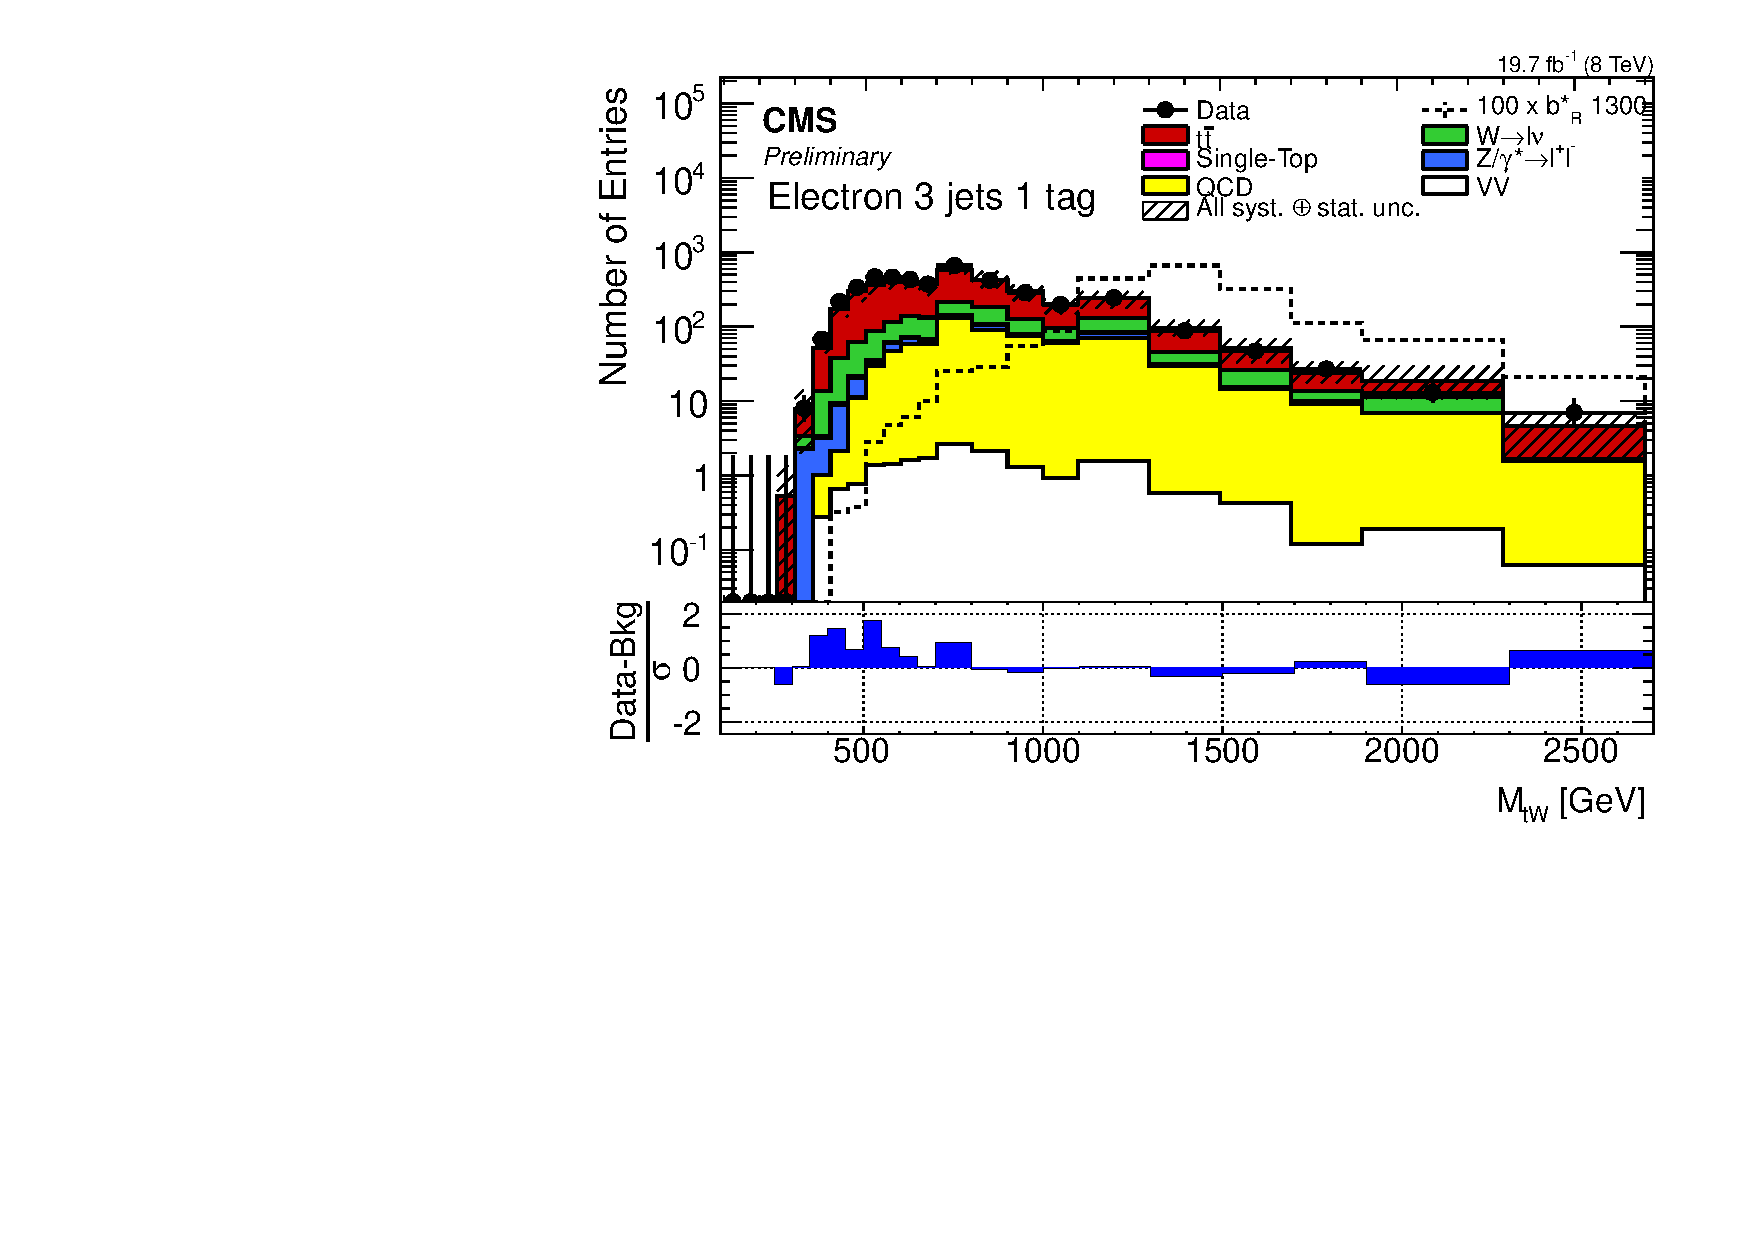
\includegraphics[width=0.6\textwidth]{AN-14-049/figs/bstarLeptonJetdataMC_CompEl1+j53XallJetLeptonMETMass_logy}
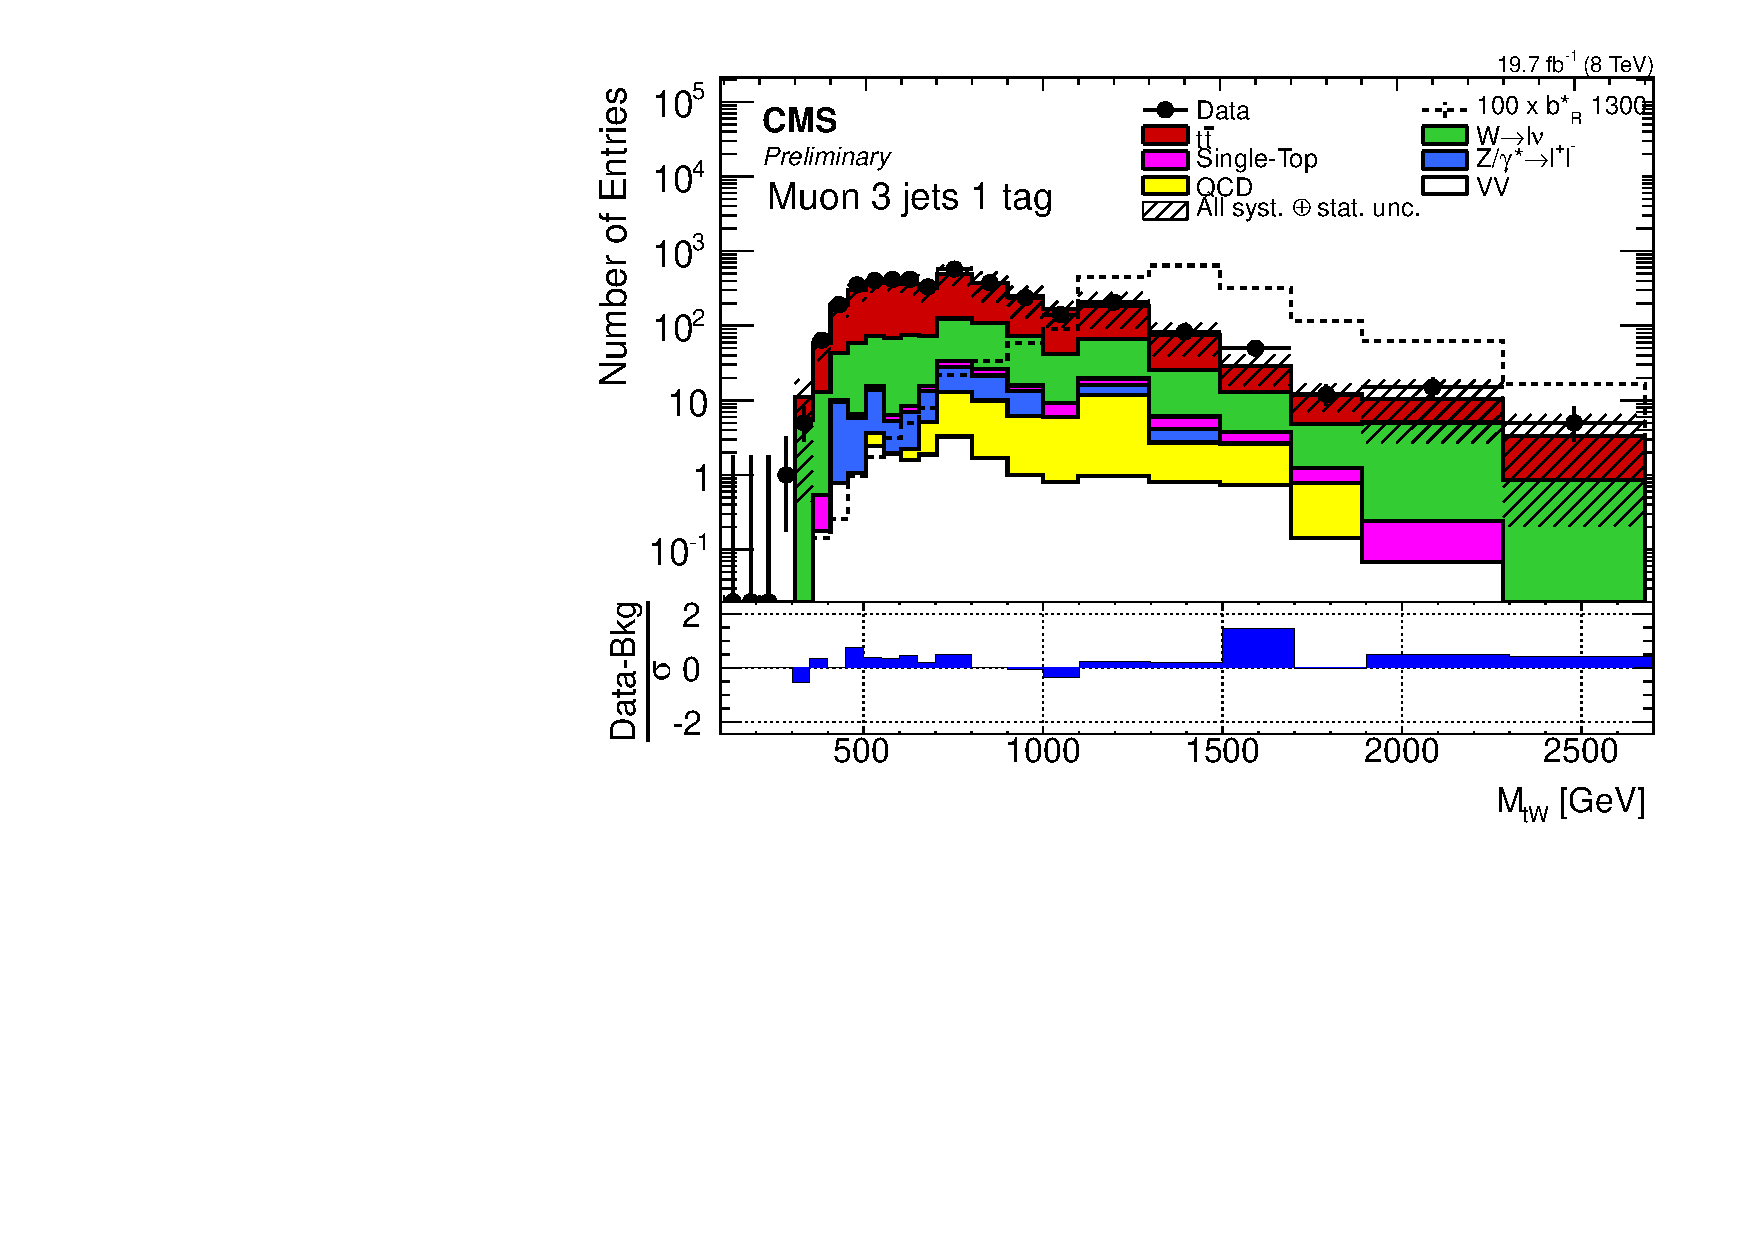
\includegraphics[width=0.6\textwidth]{AN-14-049/figs/bstarLeptonJetdataMC_CompMu1+j53XallJetLeptonMETMass_logy}
\caption{The reconstructed $\bs$ invariant mass distribution in data, background, and signal.  The channel is semileptonic in the electron+jets (top) and muon+jets(bottom). }
\label{figs:bsmtwsemi}
\end{figure}

\begin{figure}[htcb]
\centering
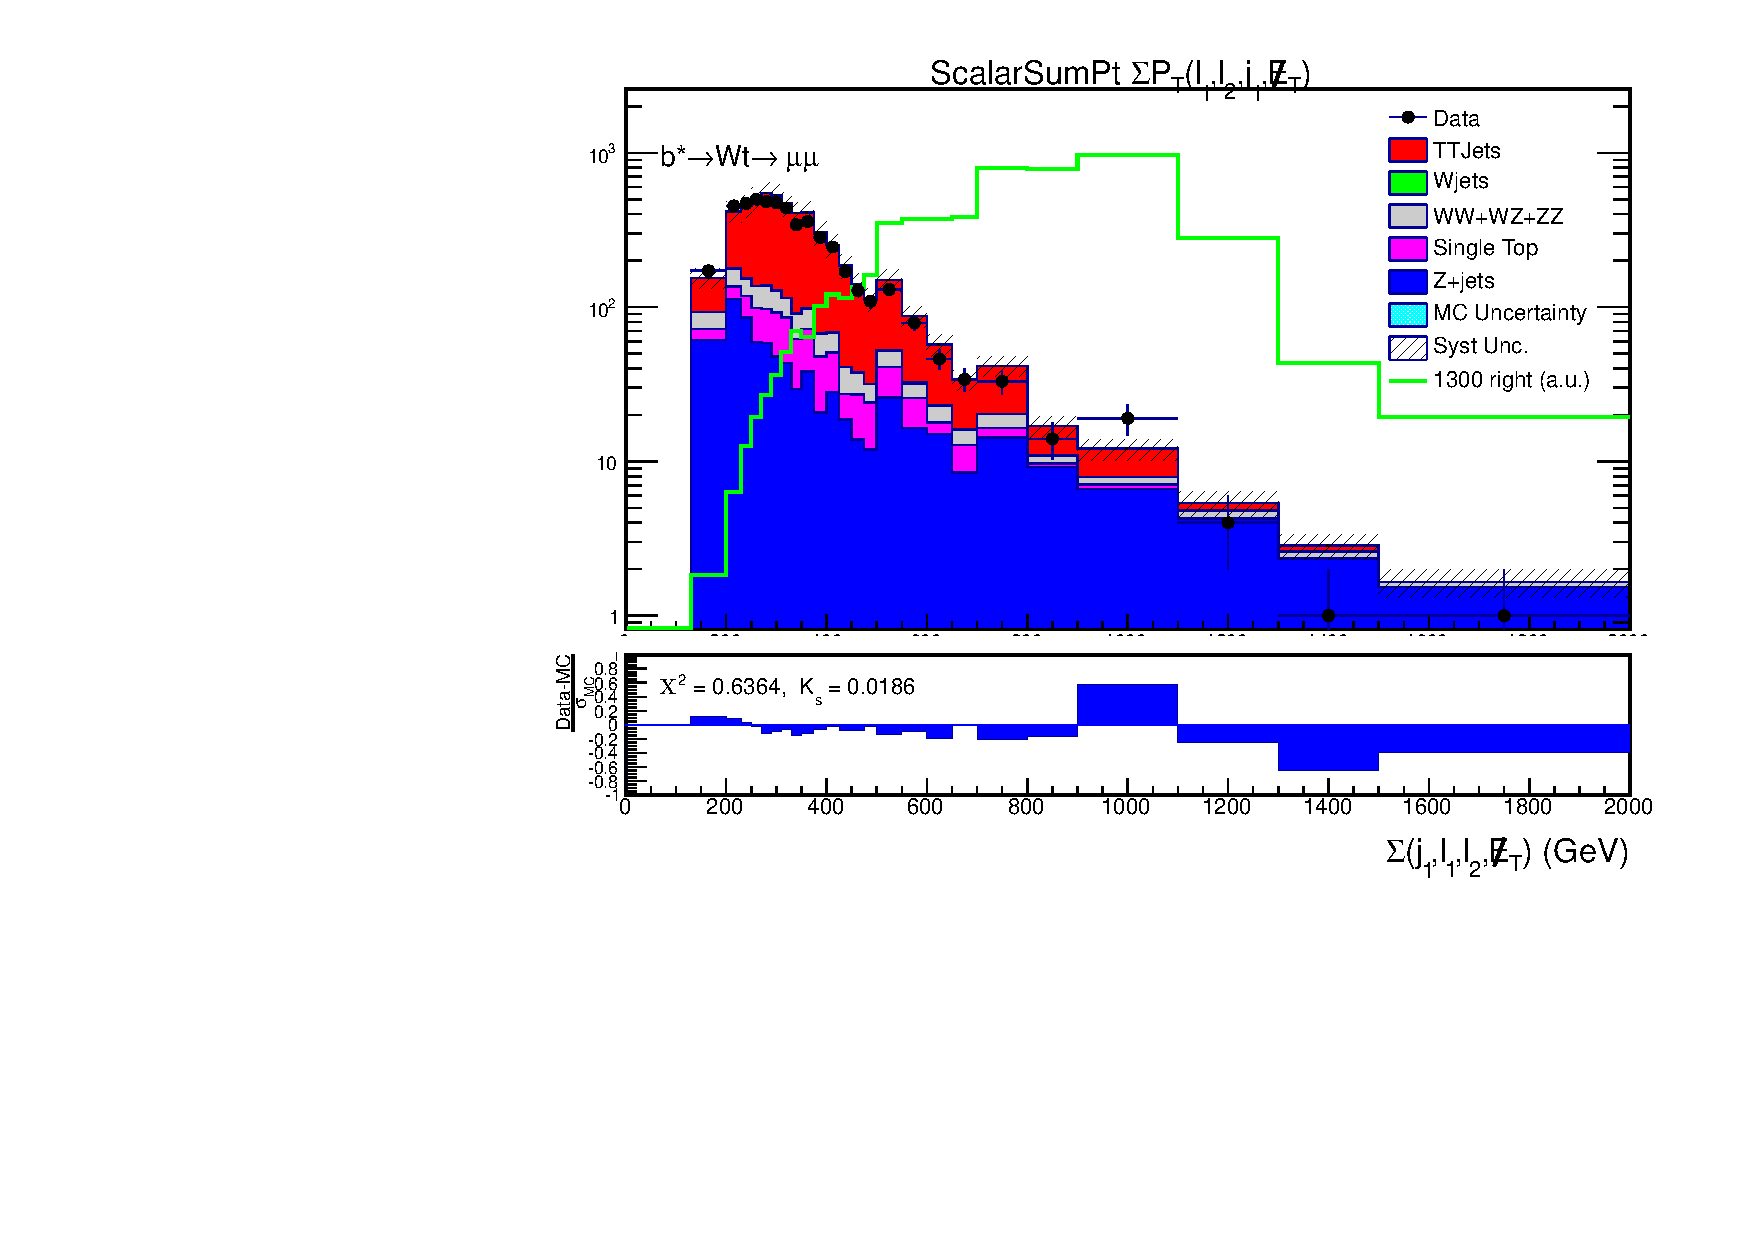
\includegraphics[width=0.6\textwidth]{AN-14-049/figs/ScalarSumPt_nGoodJetslog_mm}
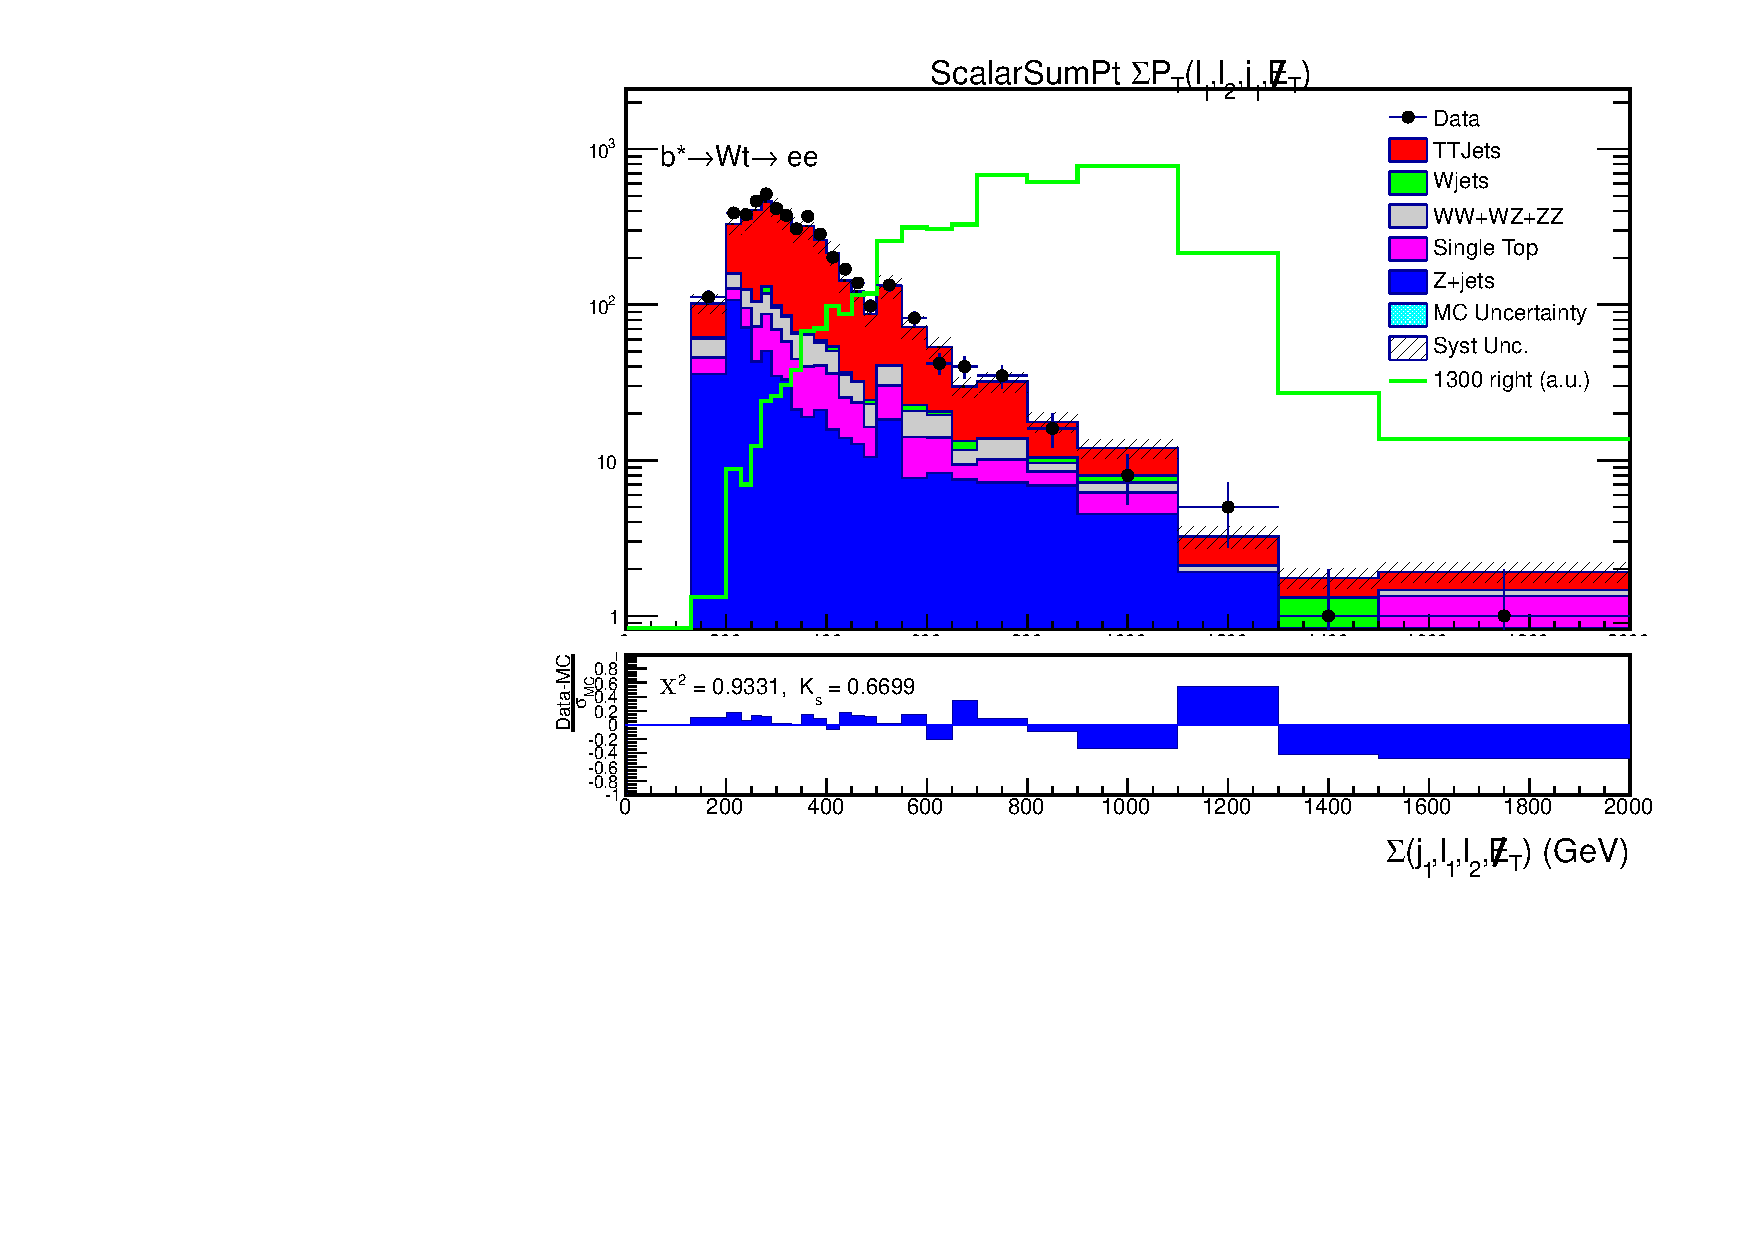
\includegraphics[width=0.6\textwidth]{AN-14-049/figs/ScalarSumPt_nGoodJetslog_ee}
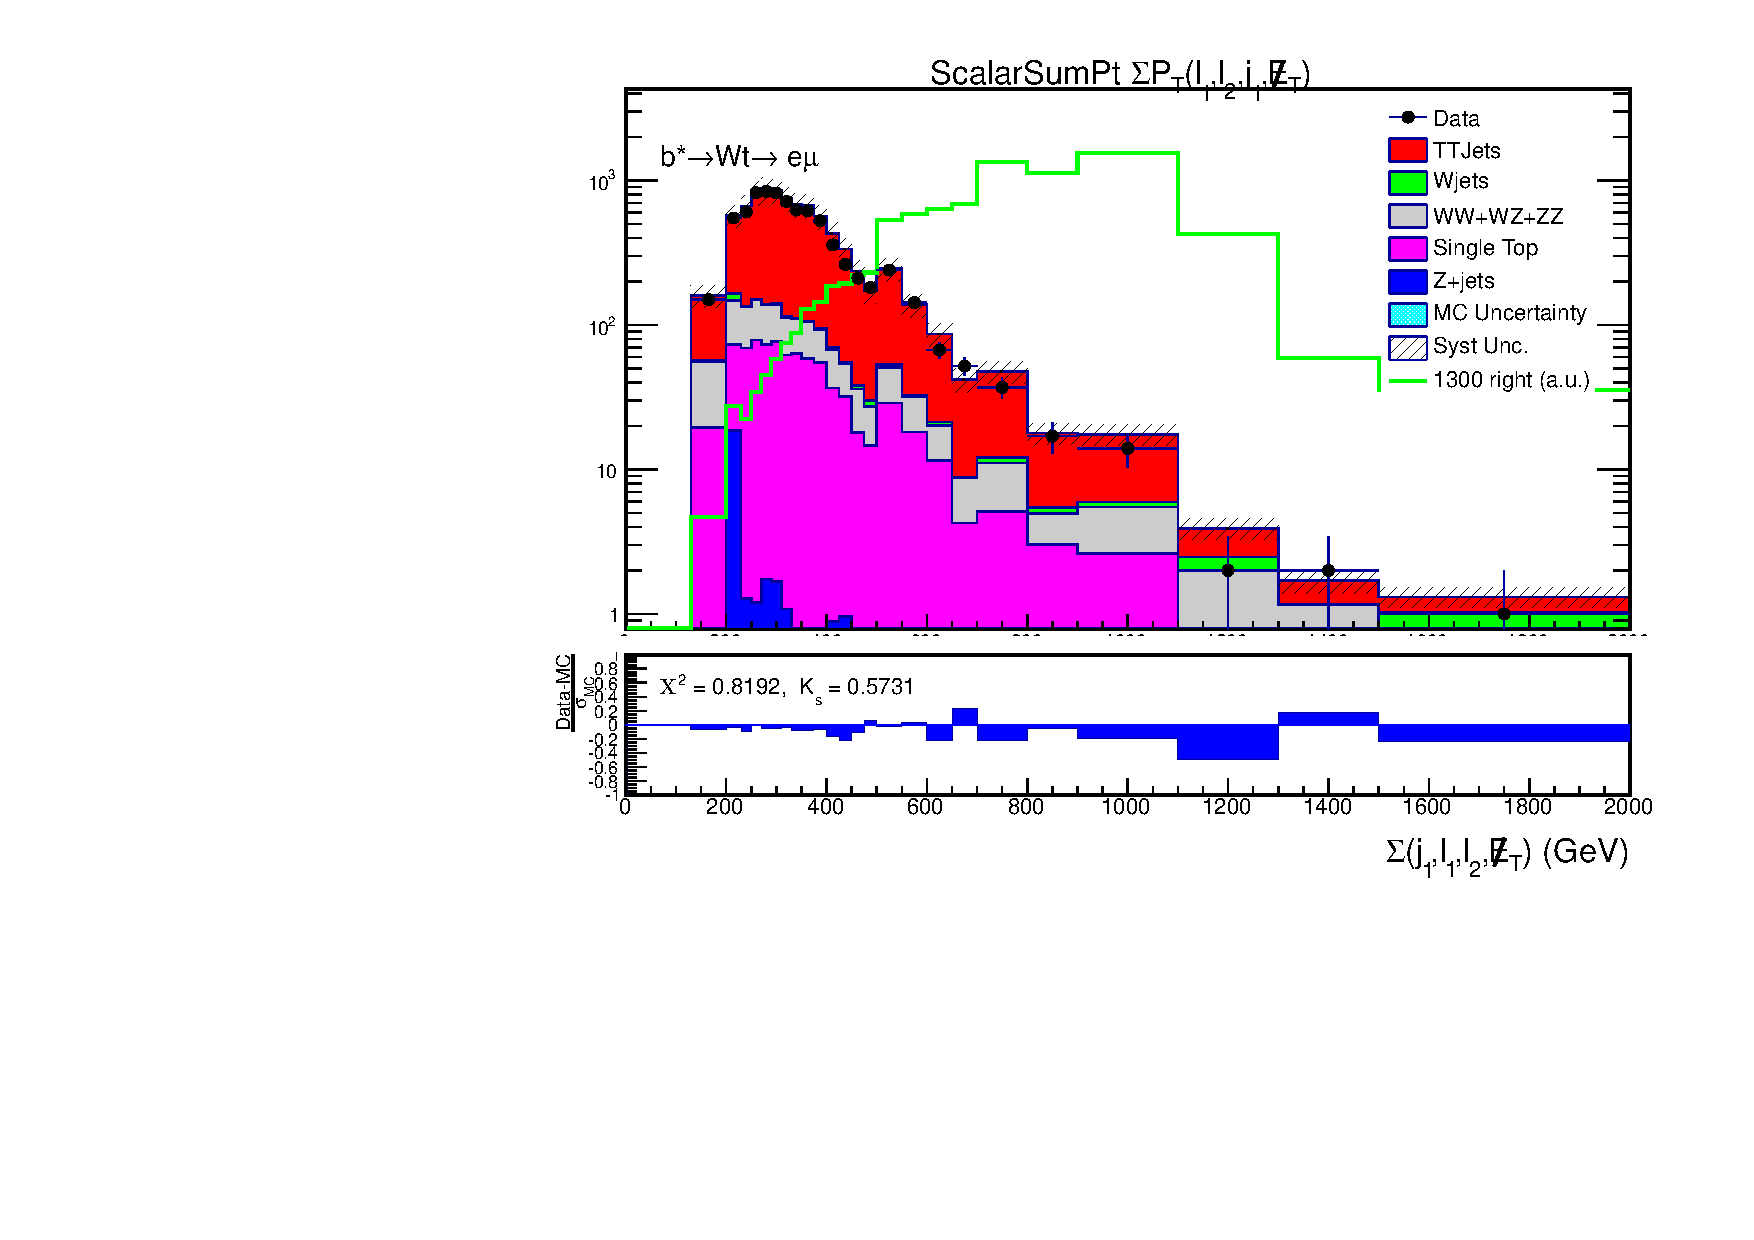
\includegraphics[width=0.6\textwidth]{AN-14-049/figs/ScalarSumPt_nGoodJetslog_em}
\caption{The reconstructed scalar $\pt$ sum distribution in data, background, and signal.  The channel is dileptonic in the muon+muon (top) electron+electron (middle) and electron+muon (bottom). }
\label{figs:bsmtwdilep}
\end{figure}

\begin{figure}[htcb]
\centering
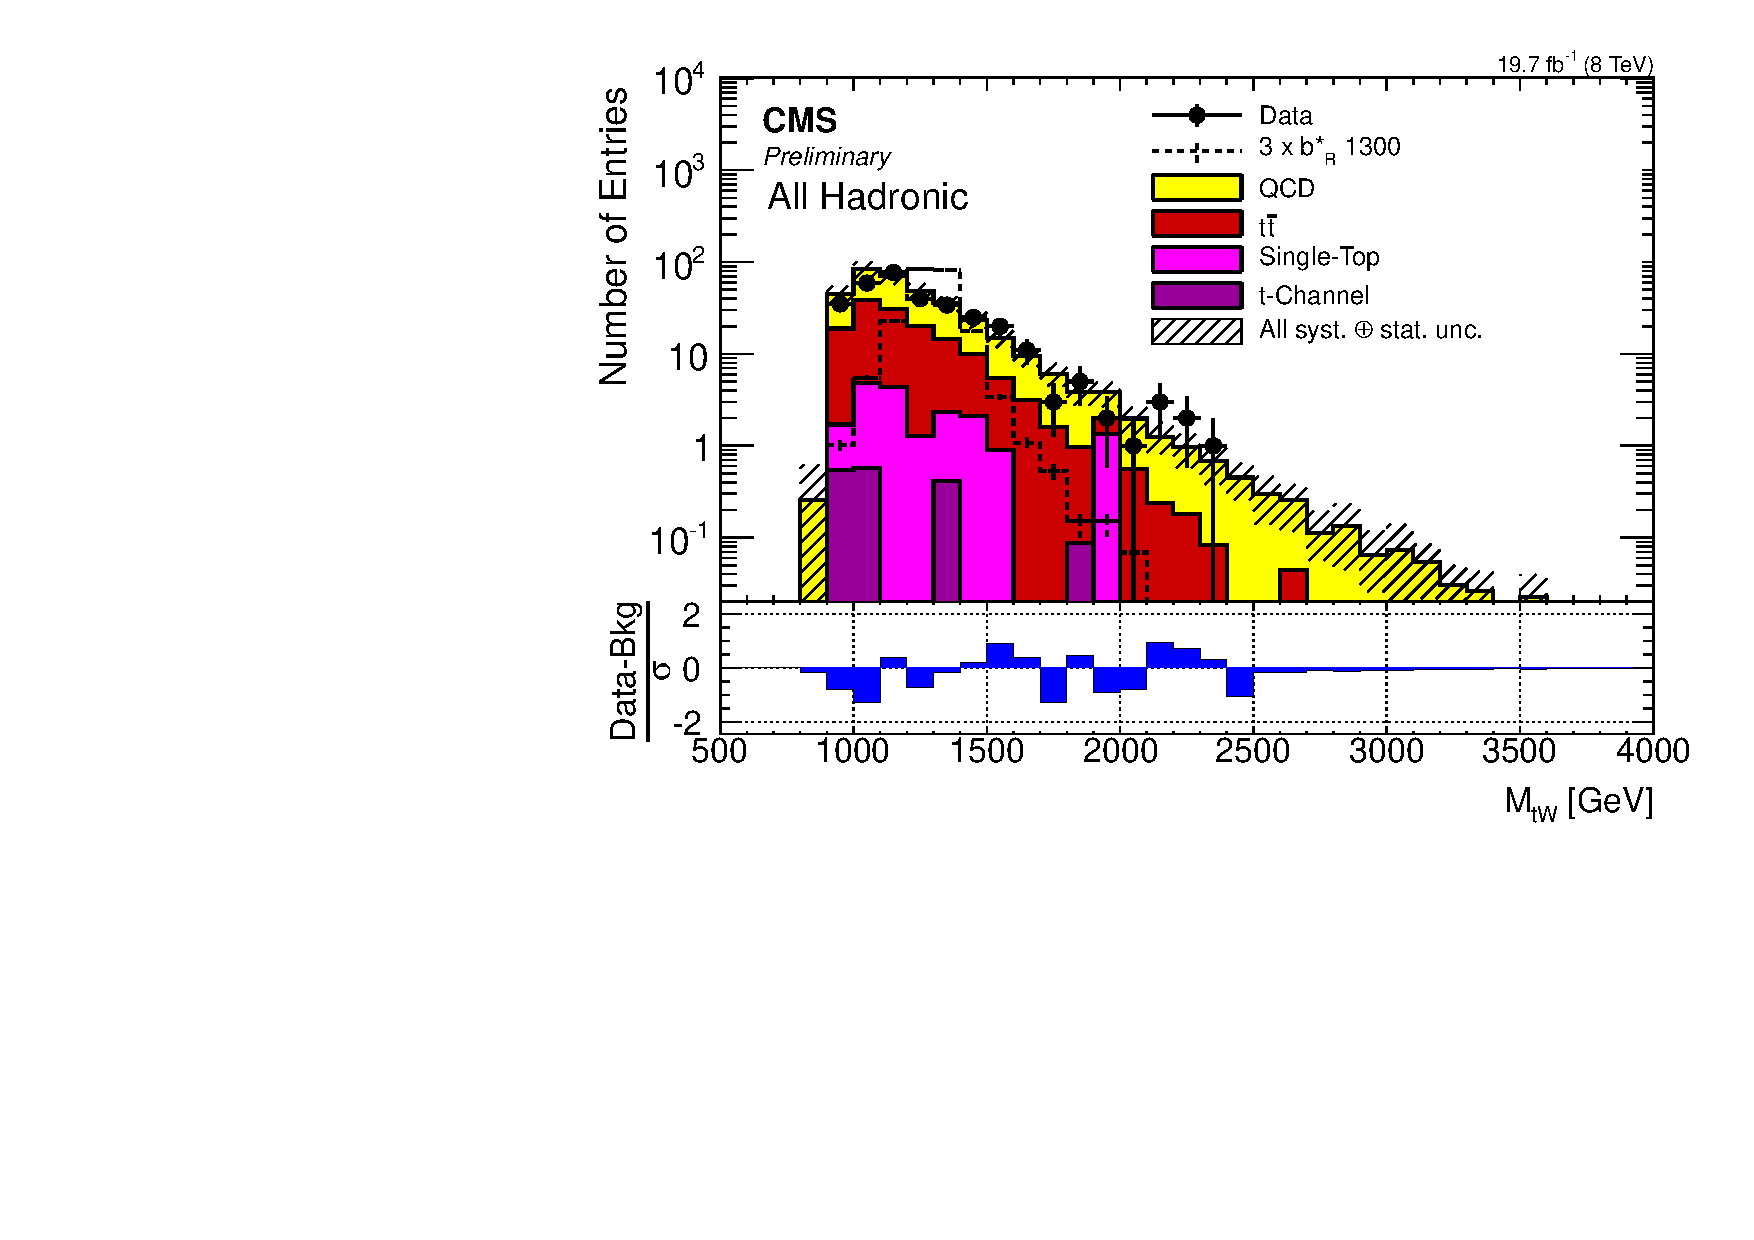
\includegraphics[width=0.6\textwidth]{AN-14-049/figs/MtwvsBkgsemilog_BifPoly_fit.pdf}
\caption{The reconstructed $\bs$ invariant mass distribution in data, background, and signal.  The channel is all-hadronic. }
\label{figs:bsmtwallhad}
\end{figure}

\begin{figure}[htcb]

\centering
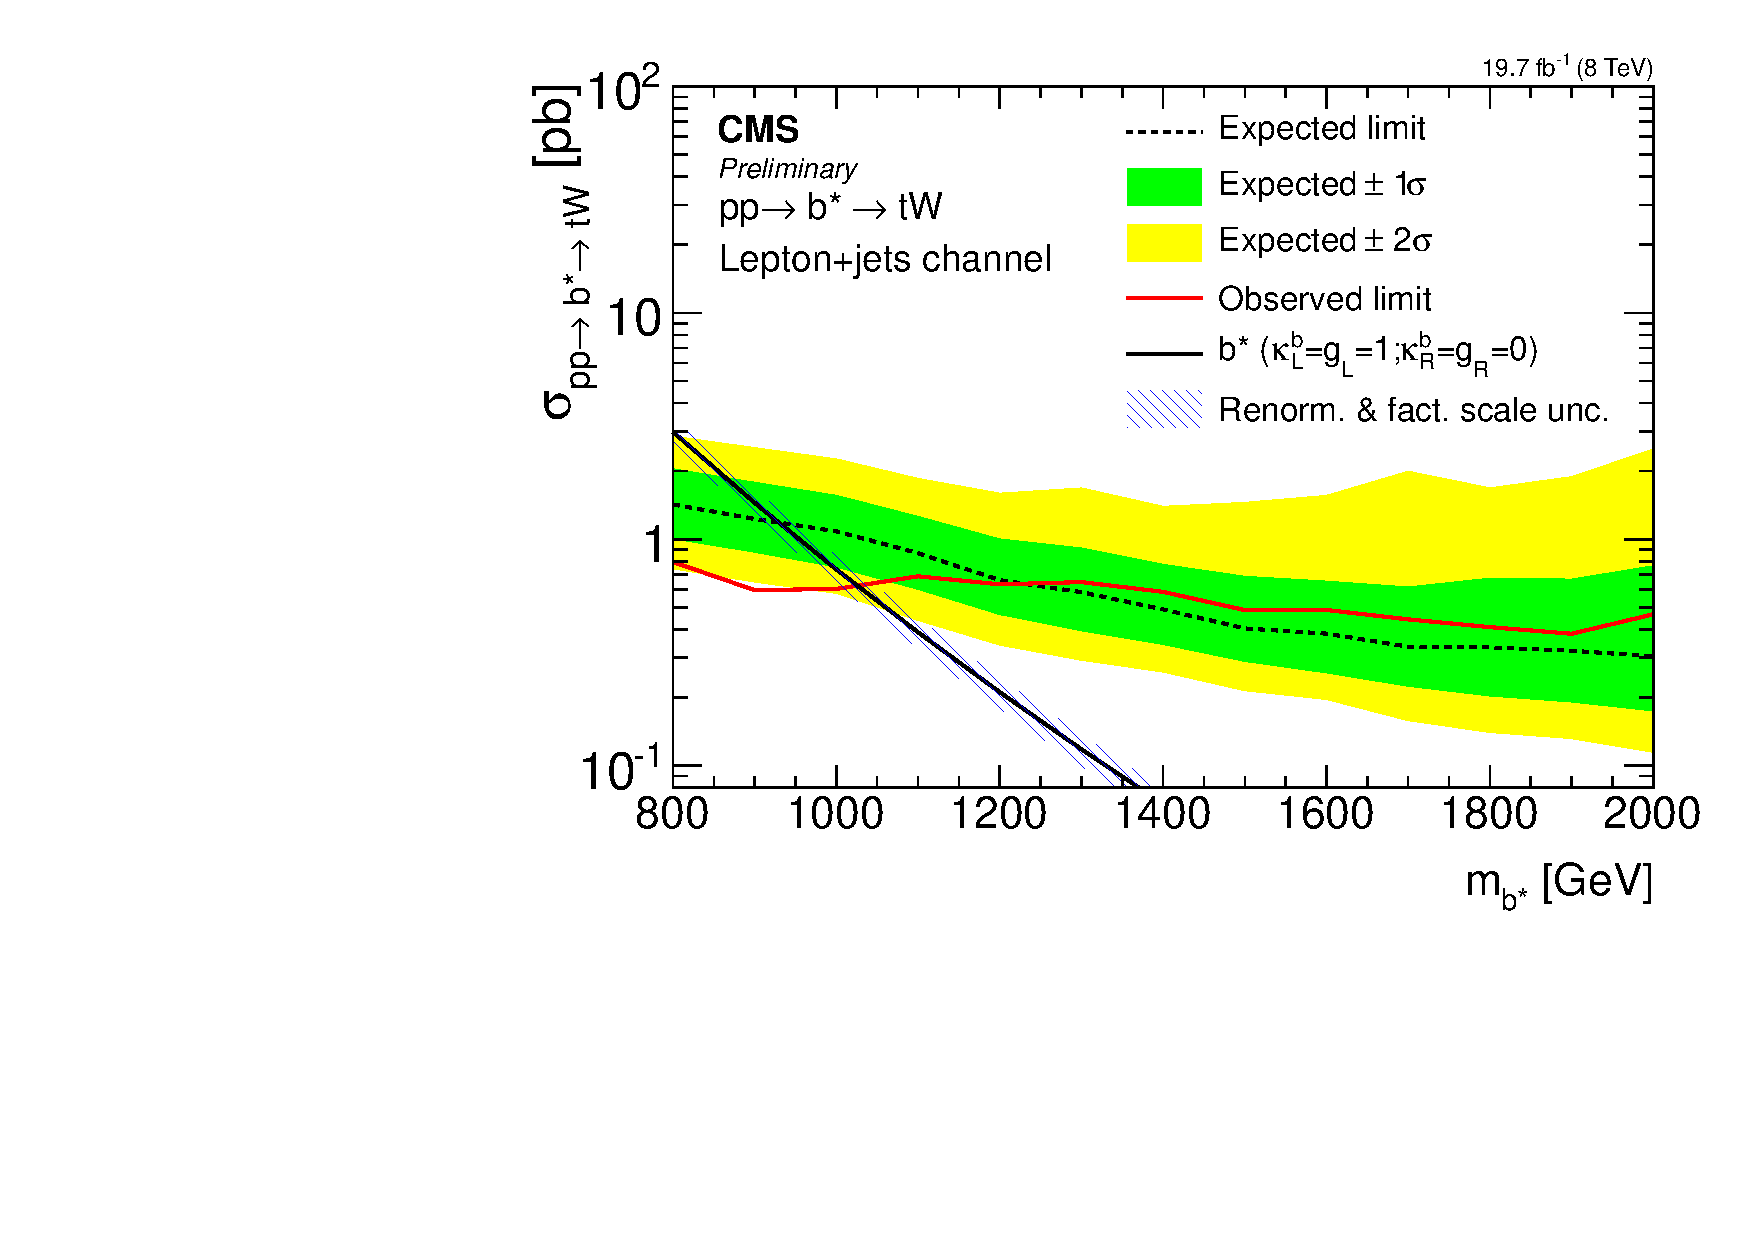
\includegraphics[width=0.6\textwidth]{AN-14-049/figs/bayesian_semileptonic_left_limit_band_plot}\\
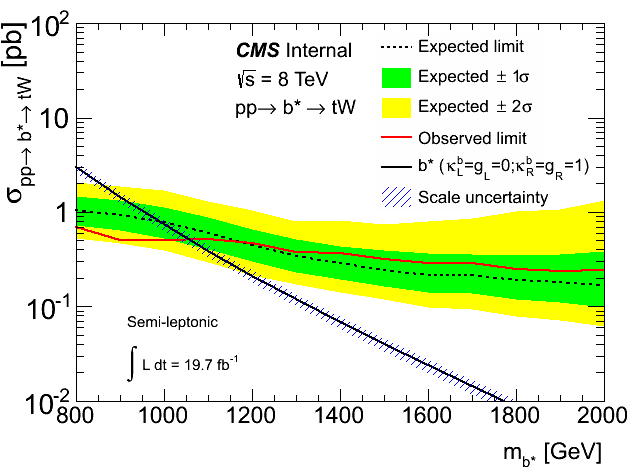
\includegraphics[width=0.6\textwidth]{AN-14-049/figs/bayesian_semileptonic_right_limit_band_plot}\\
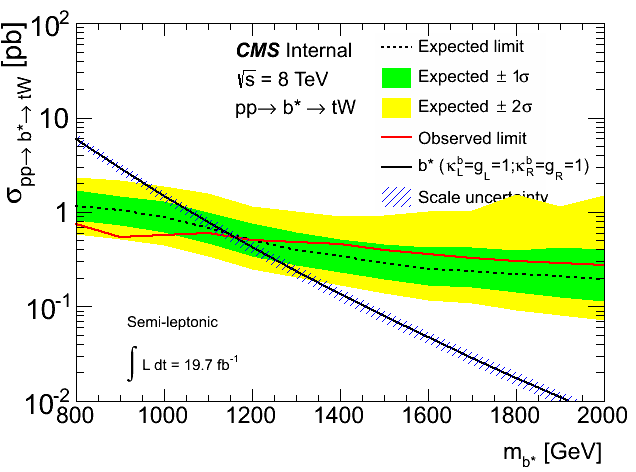
\includegraphics[width=0.6\textwidth]{AN-14-049/figs/bayesian_semileptonic_vector_limit_band_plot}
\caption{limit plot for the left-handed b* (left plot), right handed (middle plot) and vector like (right plot) $b^*$ for lepton+jets channel only. The theory error band including scale uncertainties.}
\label{figs:bslimitssemi}
\end{figure}

\begin{figure}[htcb]
\centering 
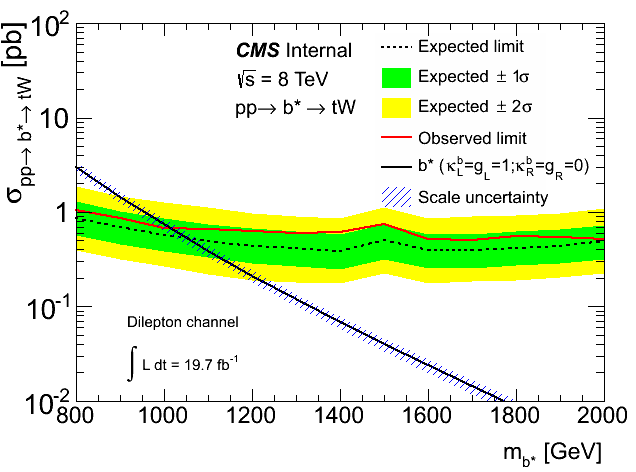
\includegraphics[width=0.6\textwidth]{AN-14-049/figs/bayesian_dileptonic_left_limit_band_plot}\\
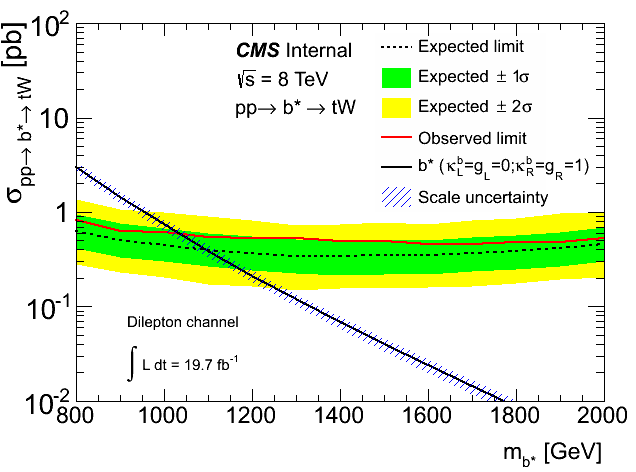
\includegraphics[width=0.6\textwidth]{AN-14-049/figs/bayesian_dileptonic_right_limit_band_plot}\\
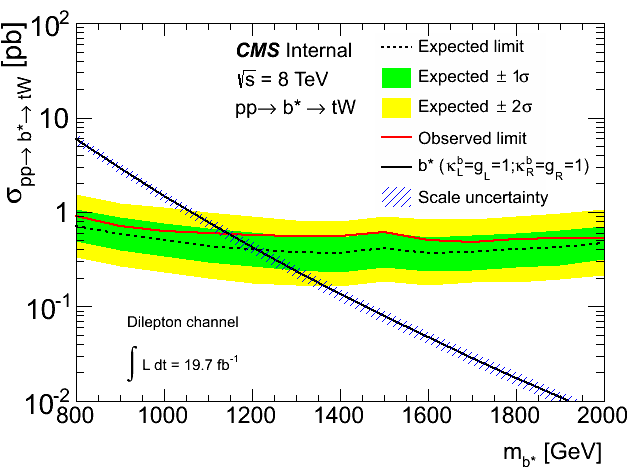
\includegraphics[width=0.6\textwidth]{AN-14-049/figs/bayesian_dileptonic_vector_limit_band_plot}
\caption{limit plot for the left-handed b* (left plot), right handed (middle plot) and vector like (right plot) $b^*$ for dilepton channel only. The theory error band including scale uncertainties.}
\label{figs:bslimitsdilep}
\end{figure}

\begin{figure}[htcb]
\centering
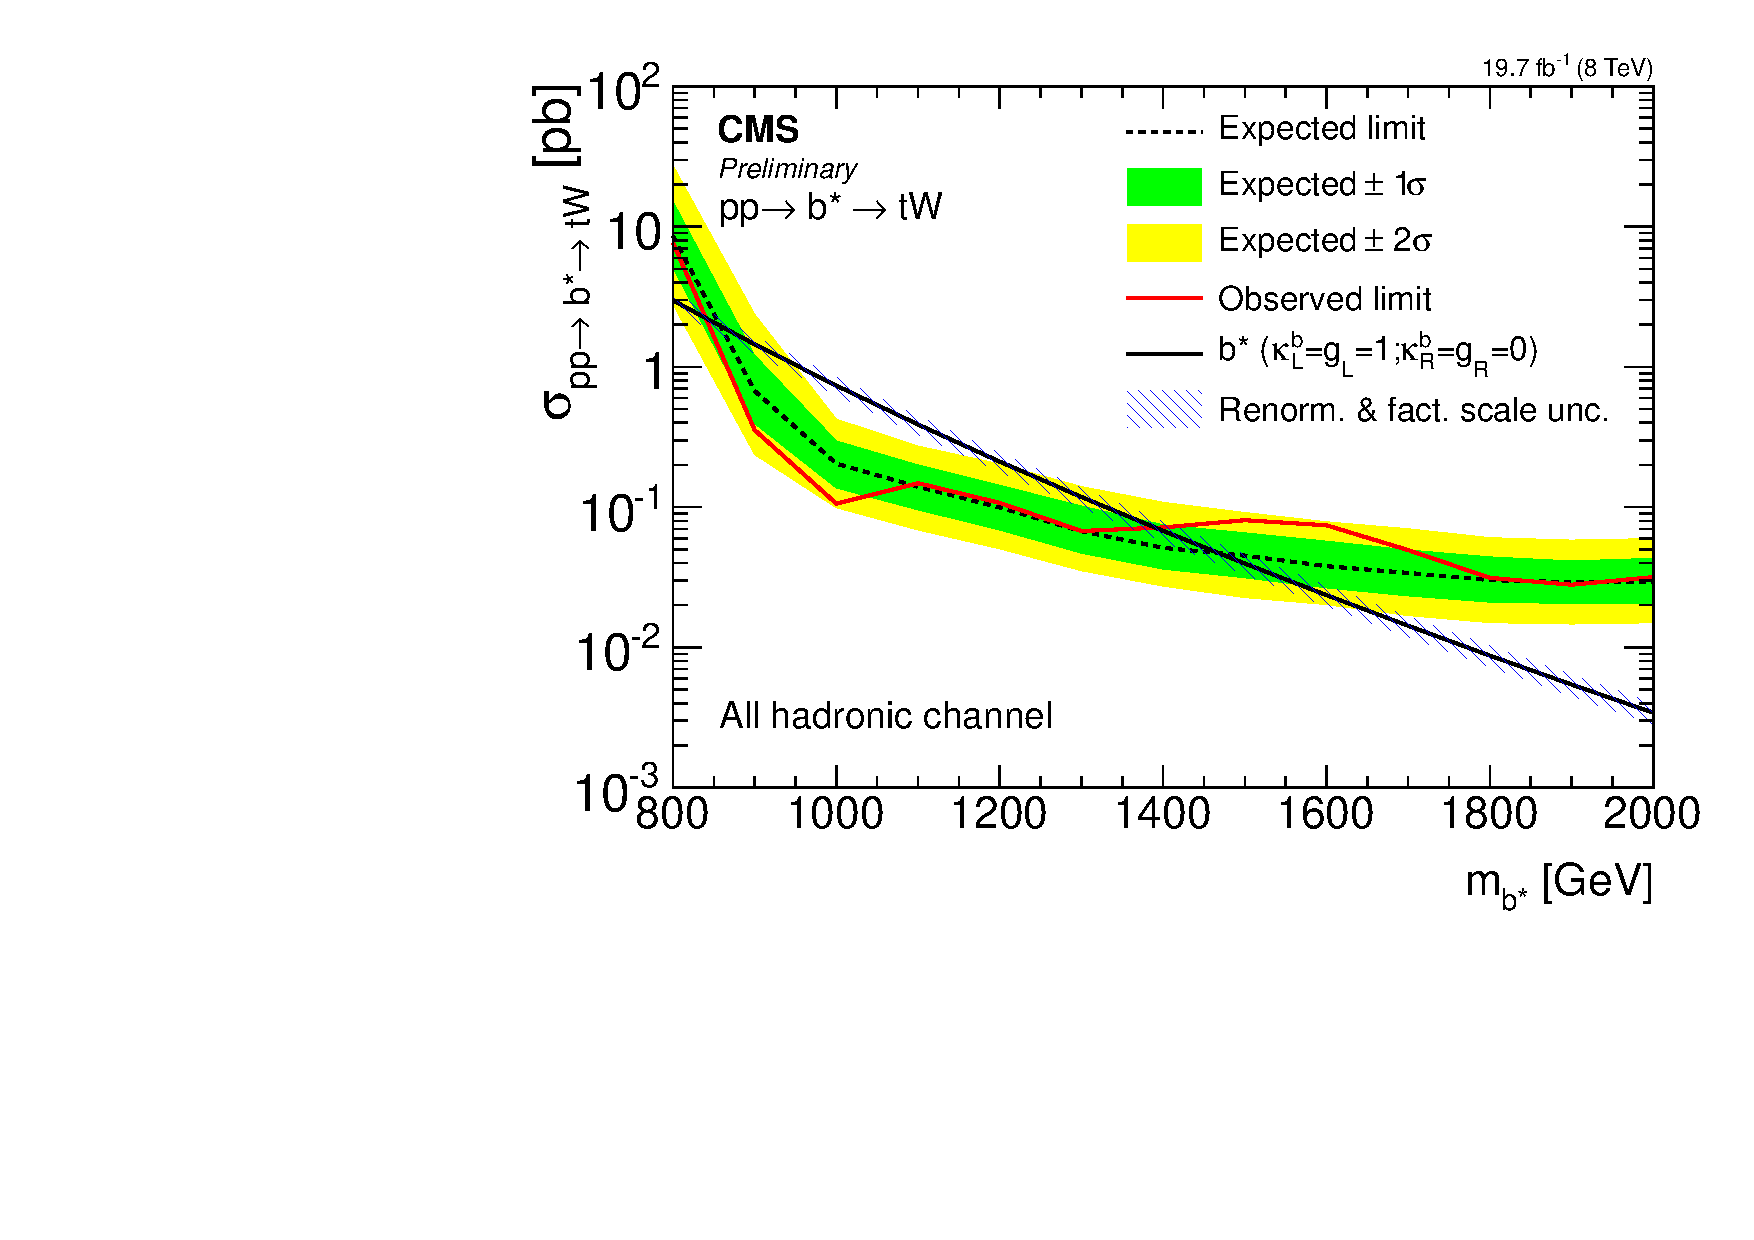
\includegraphics[width=0.6\textwidth]{AN-14-049/figs/bayesian_hadronic_left_limit_band_plot}\\
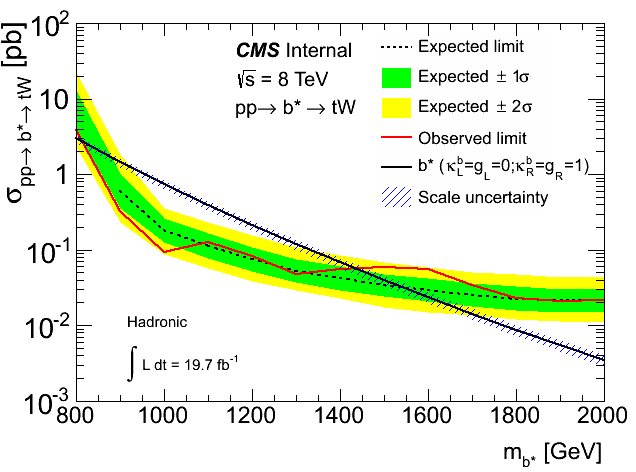
\includegraphics[width=0.6\textwidth]{AN-14-049/figs/bayesian_hadronic_right_limit_band_plot}\\
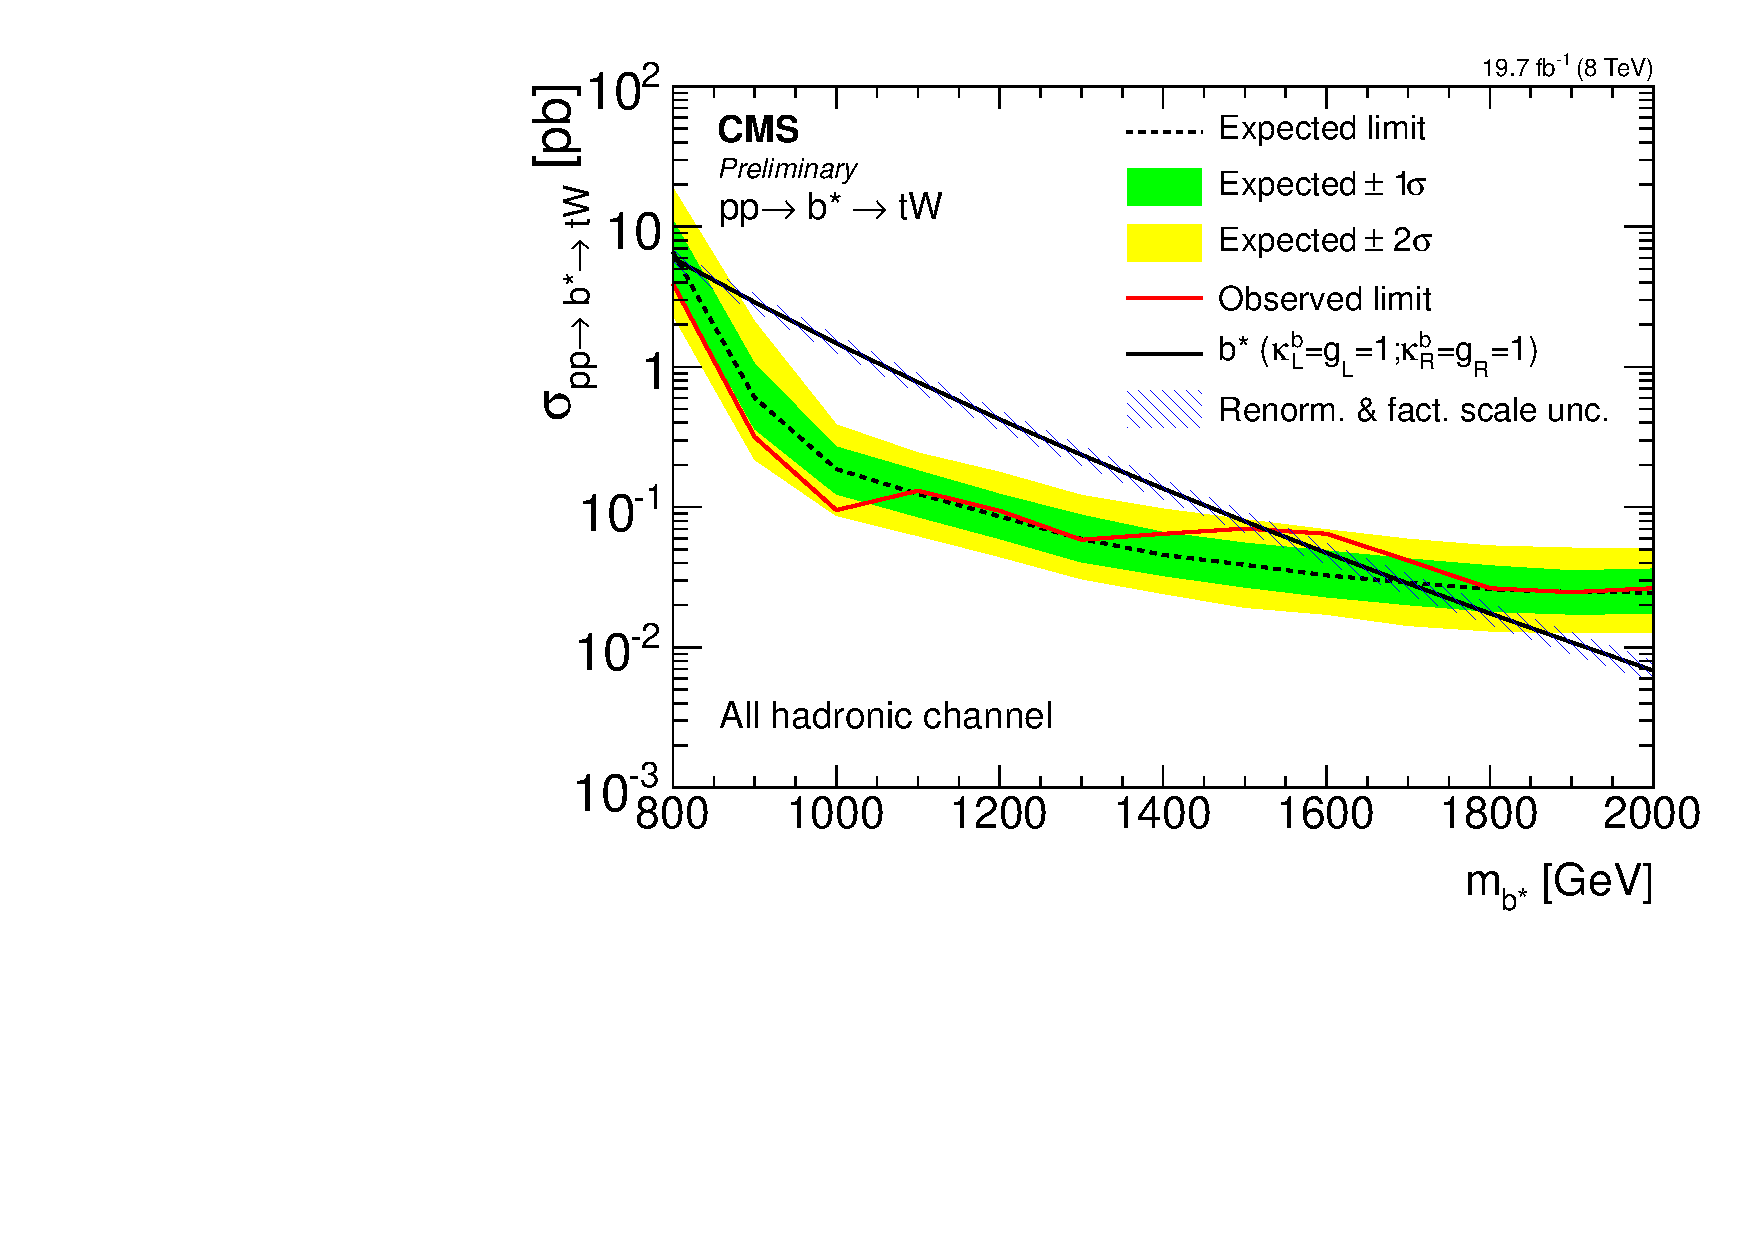
\includegraphics[width=0.6\textwidth]{AN-14-049/figs/bayesian_hadronic_vector_limit_band_plot}
\caption{limit plot for the left-handed b* (left plot), right handed (middle plot) and vector like (right plot) $b^*$ for full hadronic channel only. The theory error band including scale uncertainties.}
\label{figs:bslimitshad}
\end{figure}




The cross section upper limits can be generalized due to the fact that the $\bs$ cross-section is dependent on the unknown constants $\kappa$ and $g$.% as can be seen in equations \ref{eqn:Lag1} and \ref{eqn:Lag1}.
The limits can be extrapolated to the $g$,$\kappa$ plane as can be seen in figures \ref{figs:bsthetalimit2dobs} and \ref{figs:bsthetalimit2dexp} for observed and expected limits respectively.

The cross section upper limits for left-handed right-handed and vectorlike $\bs$ coupling hypotheses are shown in Tables \ref{table:bsupperxsecL} \ref{table:bsupperxsecR} and \ref{table:bsupperxsecLR} respectively.

The $\bs$ mass exclusion point for each channel is given in table \ref{limitTable}





\begin{figure}[htcb]
\centering
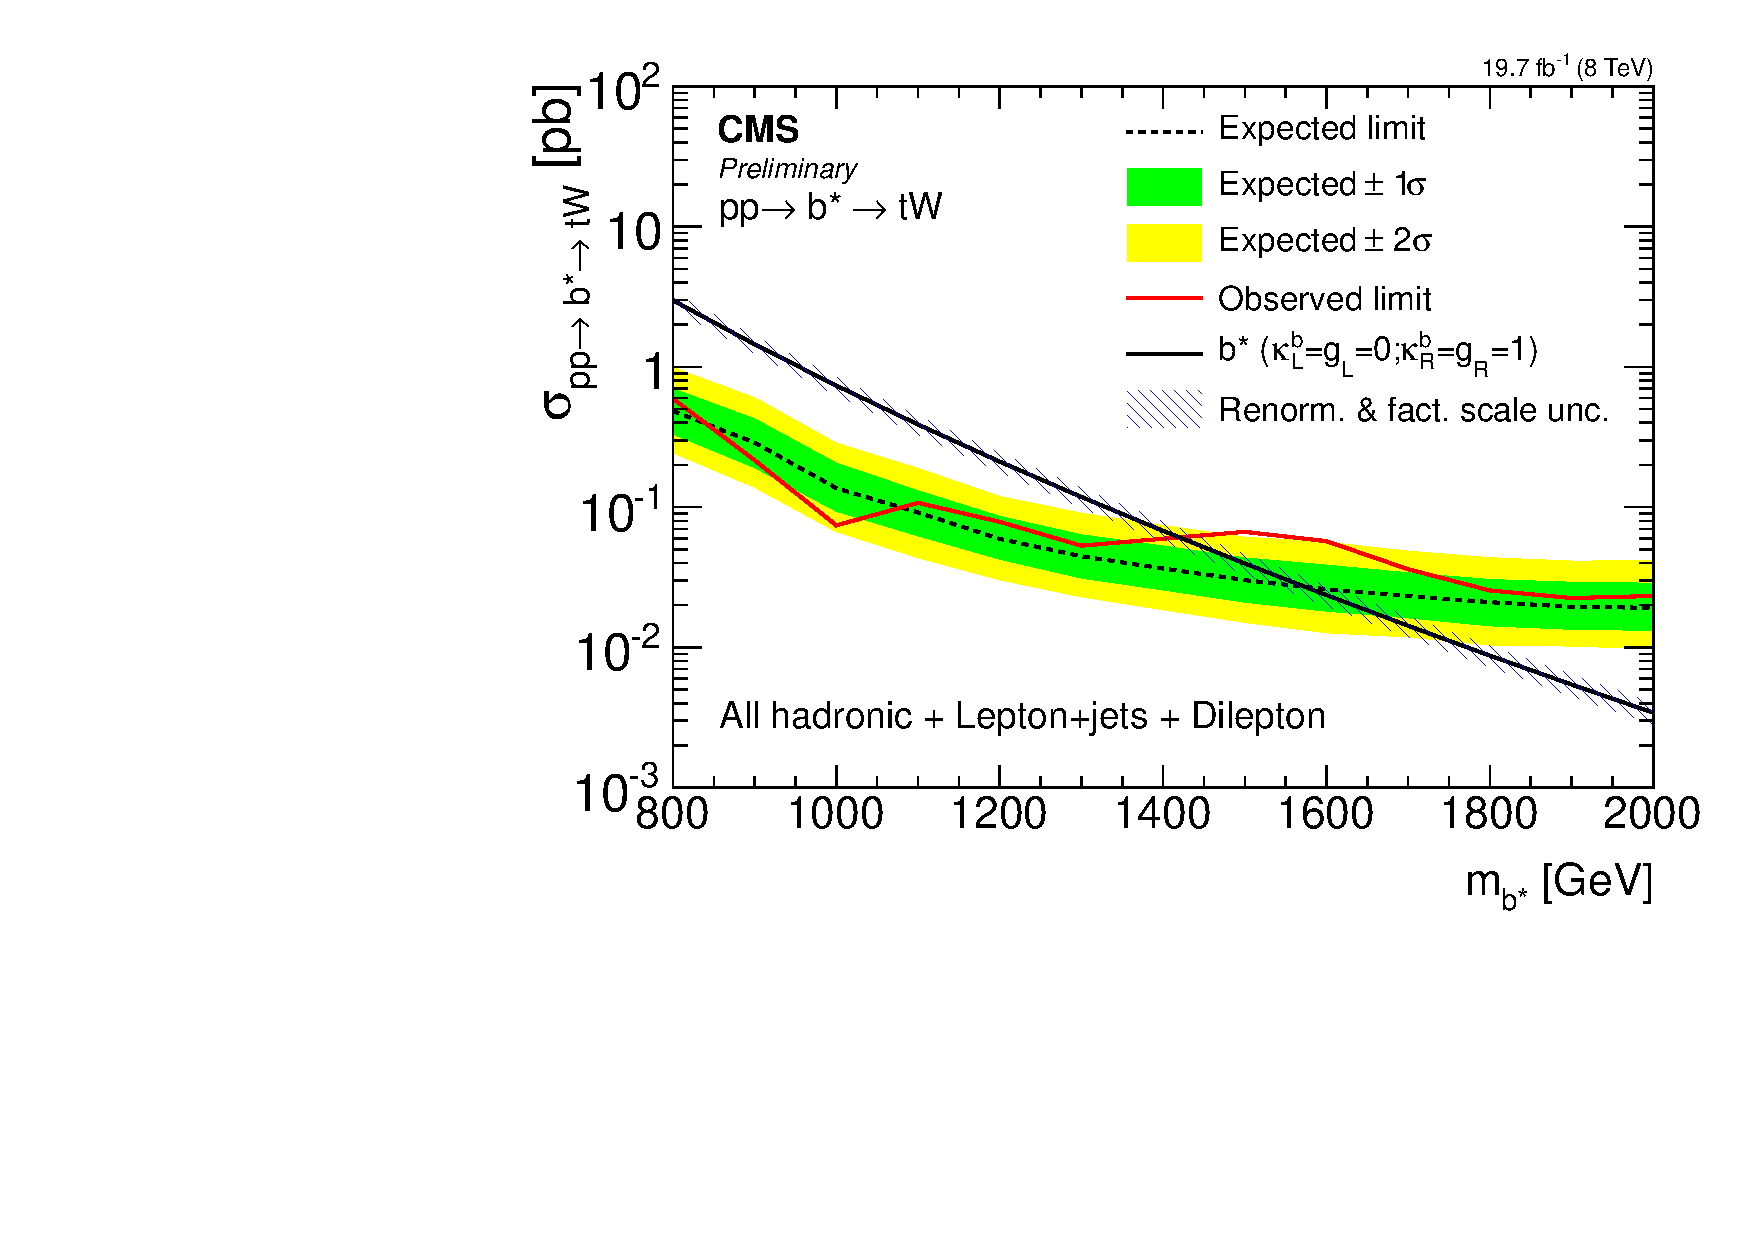
\includegraphics[width=0.5\textwidth]{AN-14-049/figs/bayesian_hadronic_semileptonic_right_limit_band_plot.pdf}\\
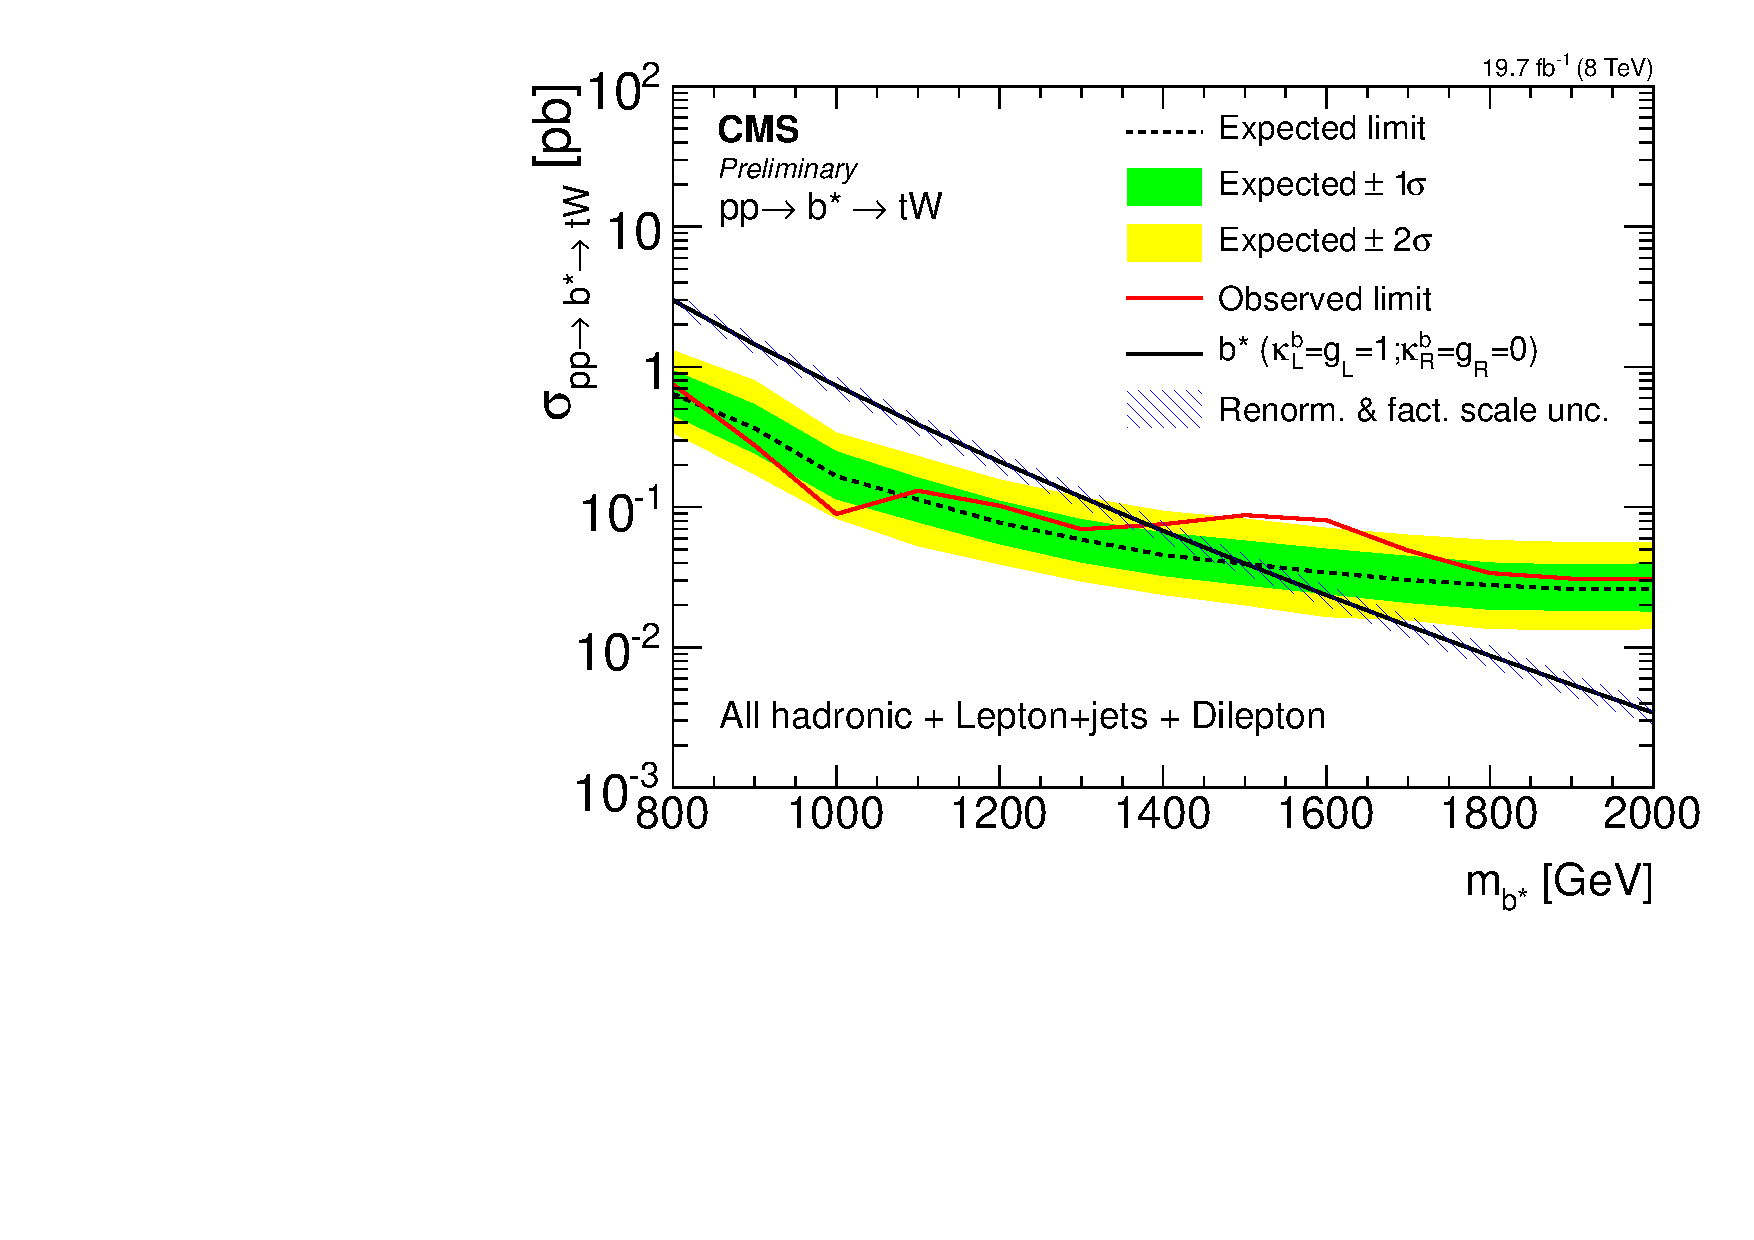
\includegraphics[width=0.5\textwidth]{AN-14-049/figs/bayesian_hadronic_semileptonic_left_limit_band_plot.pdf}\\
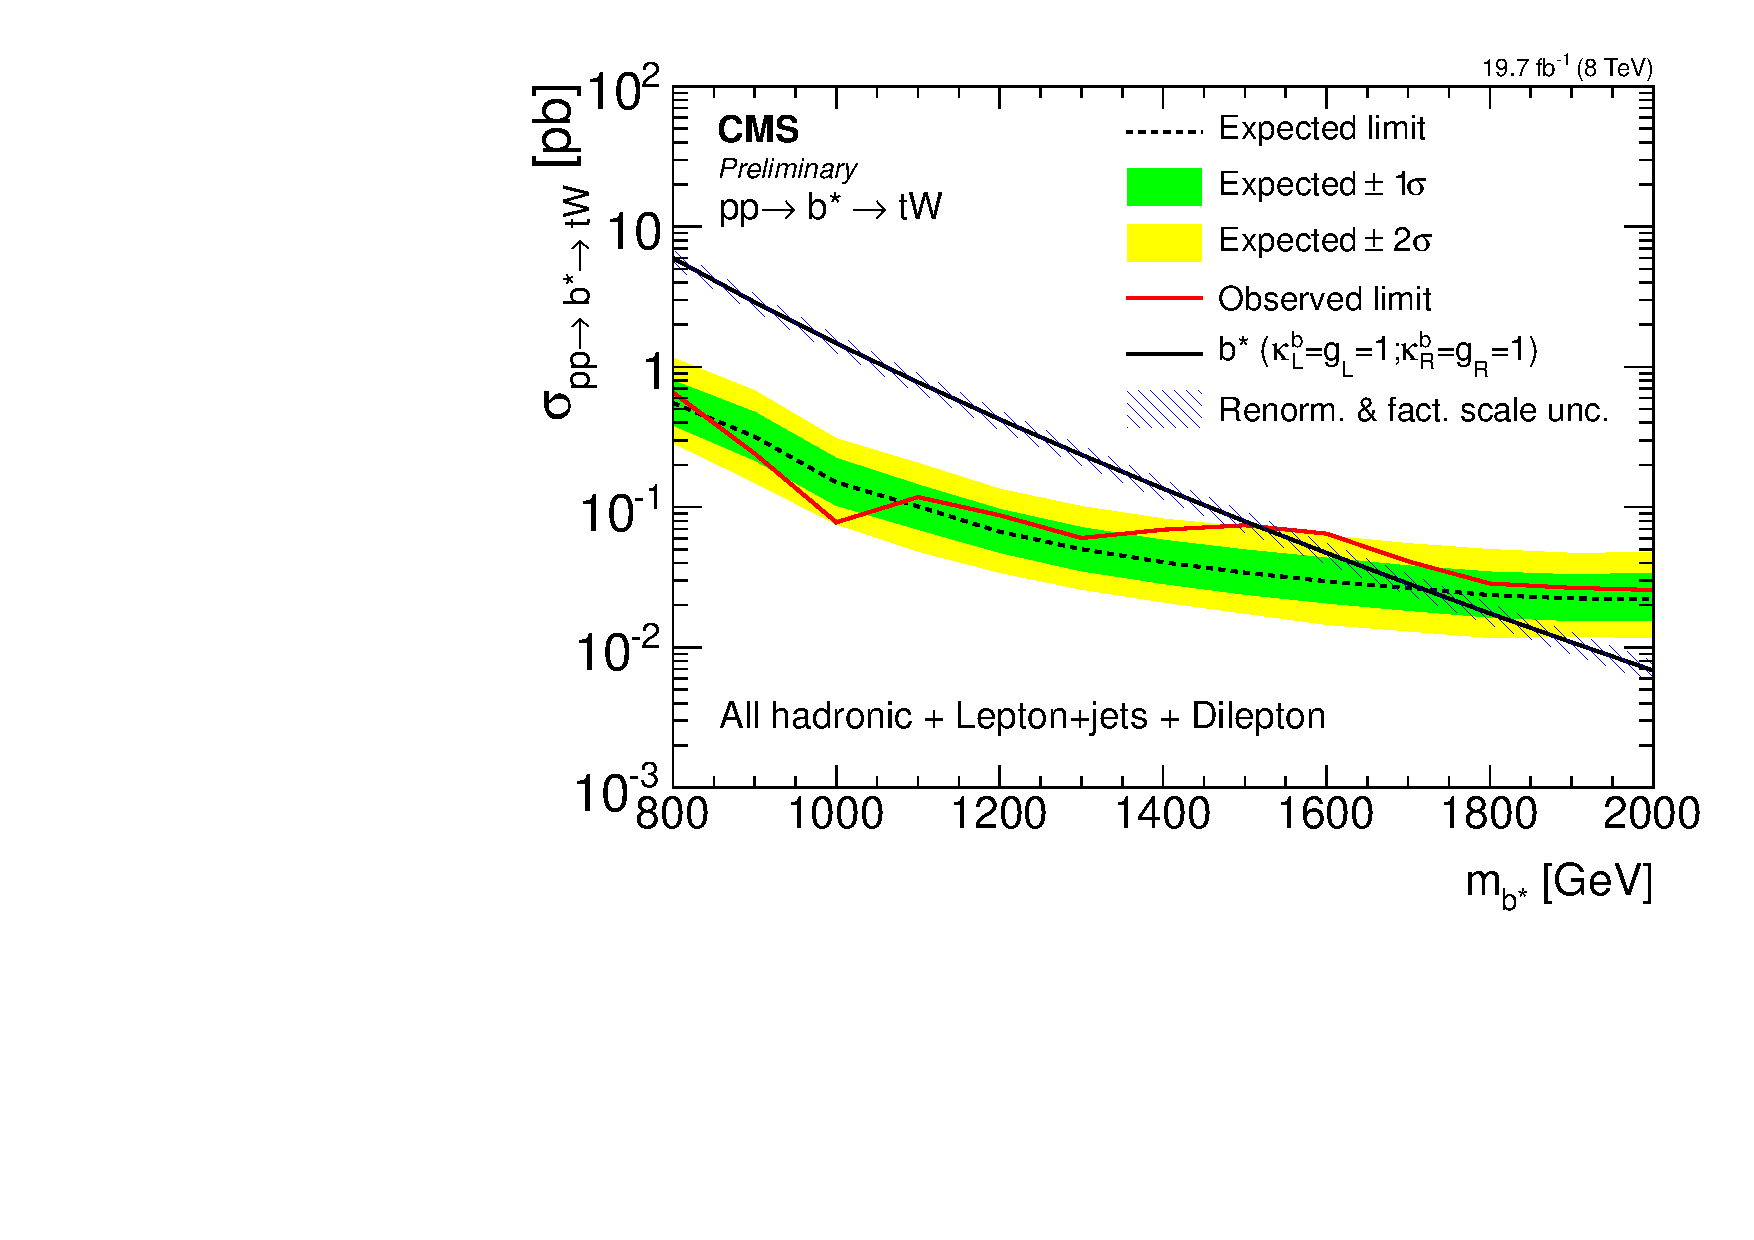
\includegraphics[width=0.5\textwidth]{AN-14-049/figs/bayesian_hadronic_semileptonic_vector_limit_band_plot.pdf}
\caption{The $\bs$ quark 95\% C.L. production cross-section limits.  The expected (black) and observed (red) limits as well as $\bs$ quark 
theoretical cross-section (blue) are plotted for comparison.  
The uncertainty in the expected limit band is shown in light ($\pm$1$\sigma$) and dark grey ($\pm$2$\sigma$).
These limits were extracted using the Theta limit setting framework.  Here, the signal hypotheses of a right-handed, left-handed, and vector-like $\bs$ quark are 
shown on the top, middle, and bottom plots respectively. }
\label{figs:bsthetalimit}
\end{figure}

\begin{figure}[htcb]
\centering
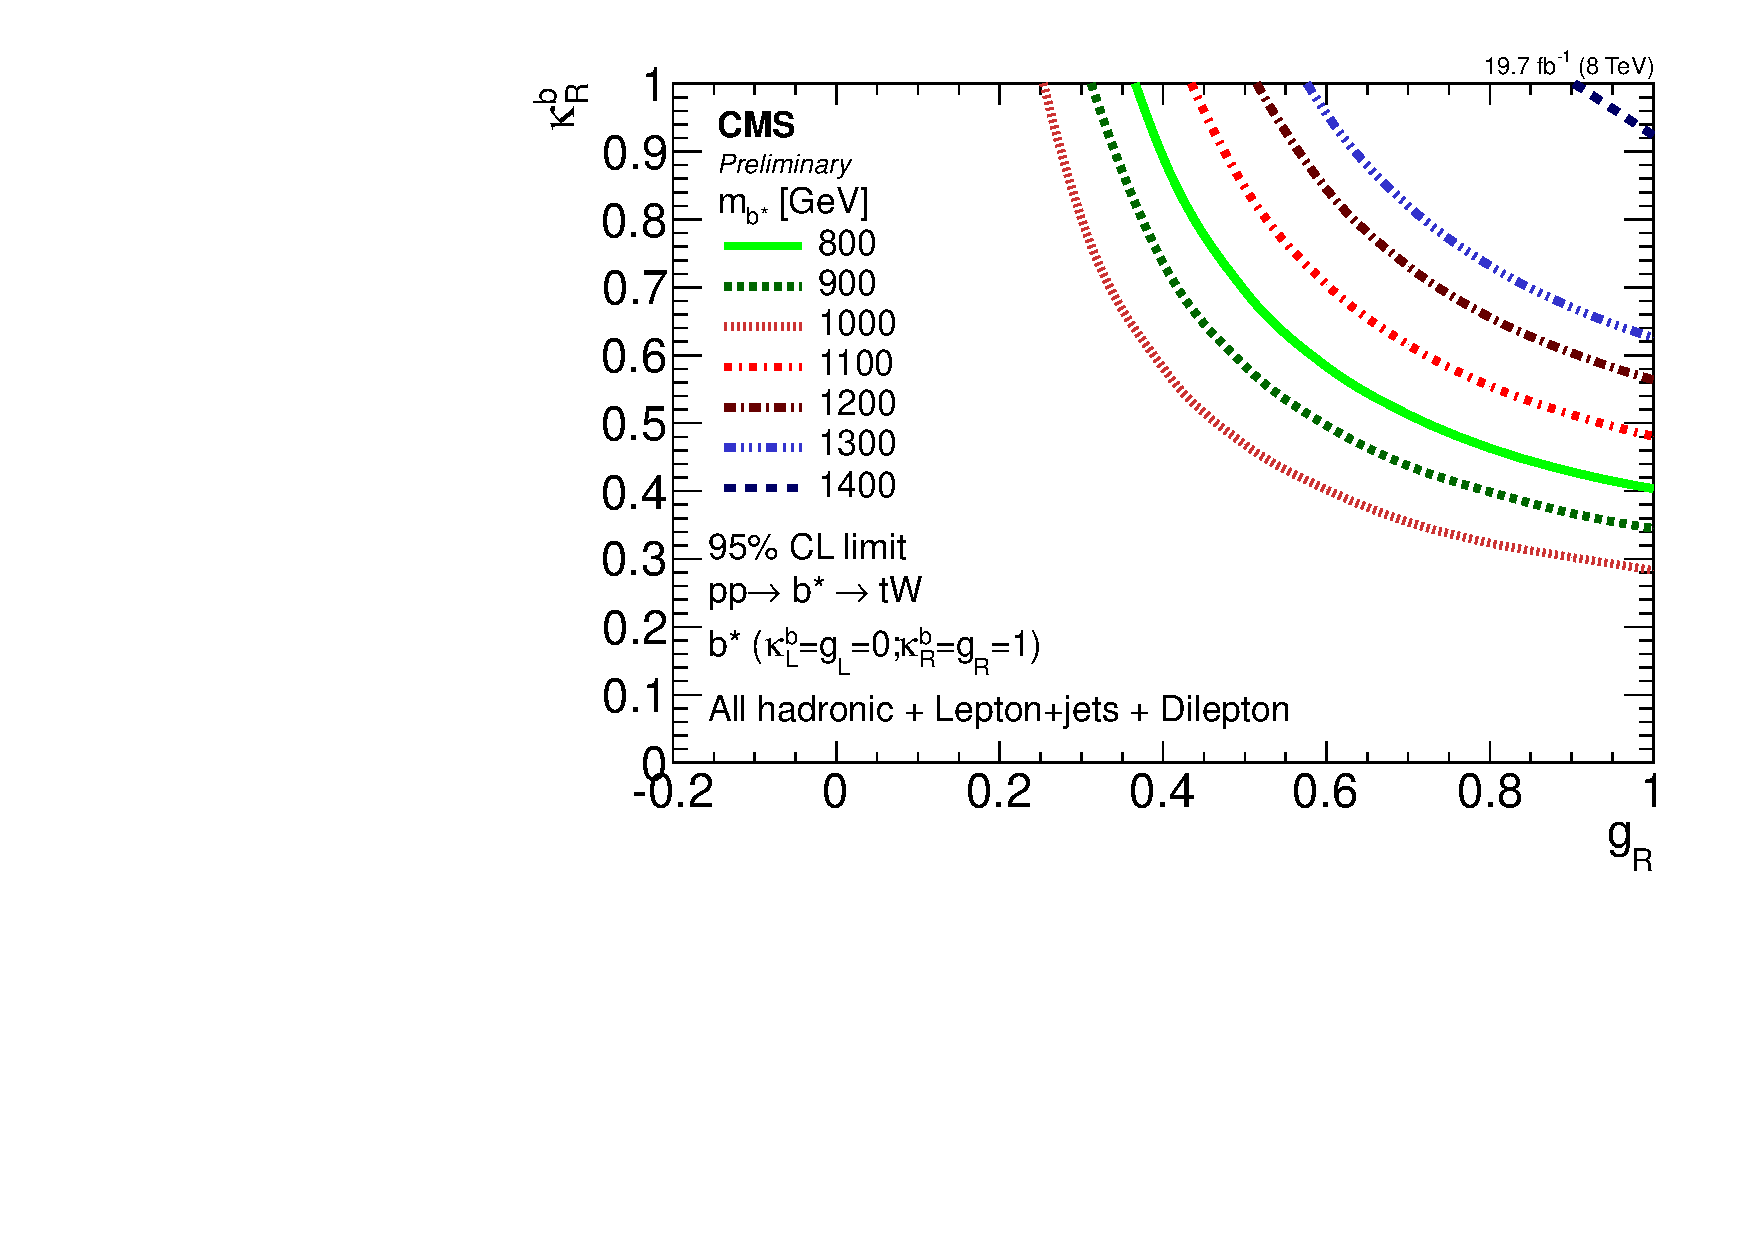
\includegraphics[width=0.6\textwidth]{AN-14-049/figs/bayesian_observed_hadronic_semileptonic_right_2Dlimit_plot.pdf}\\
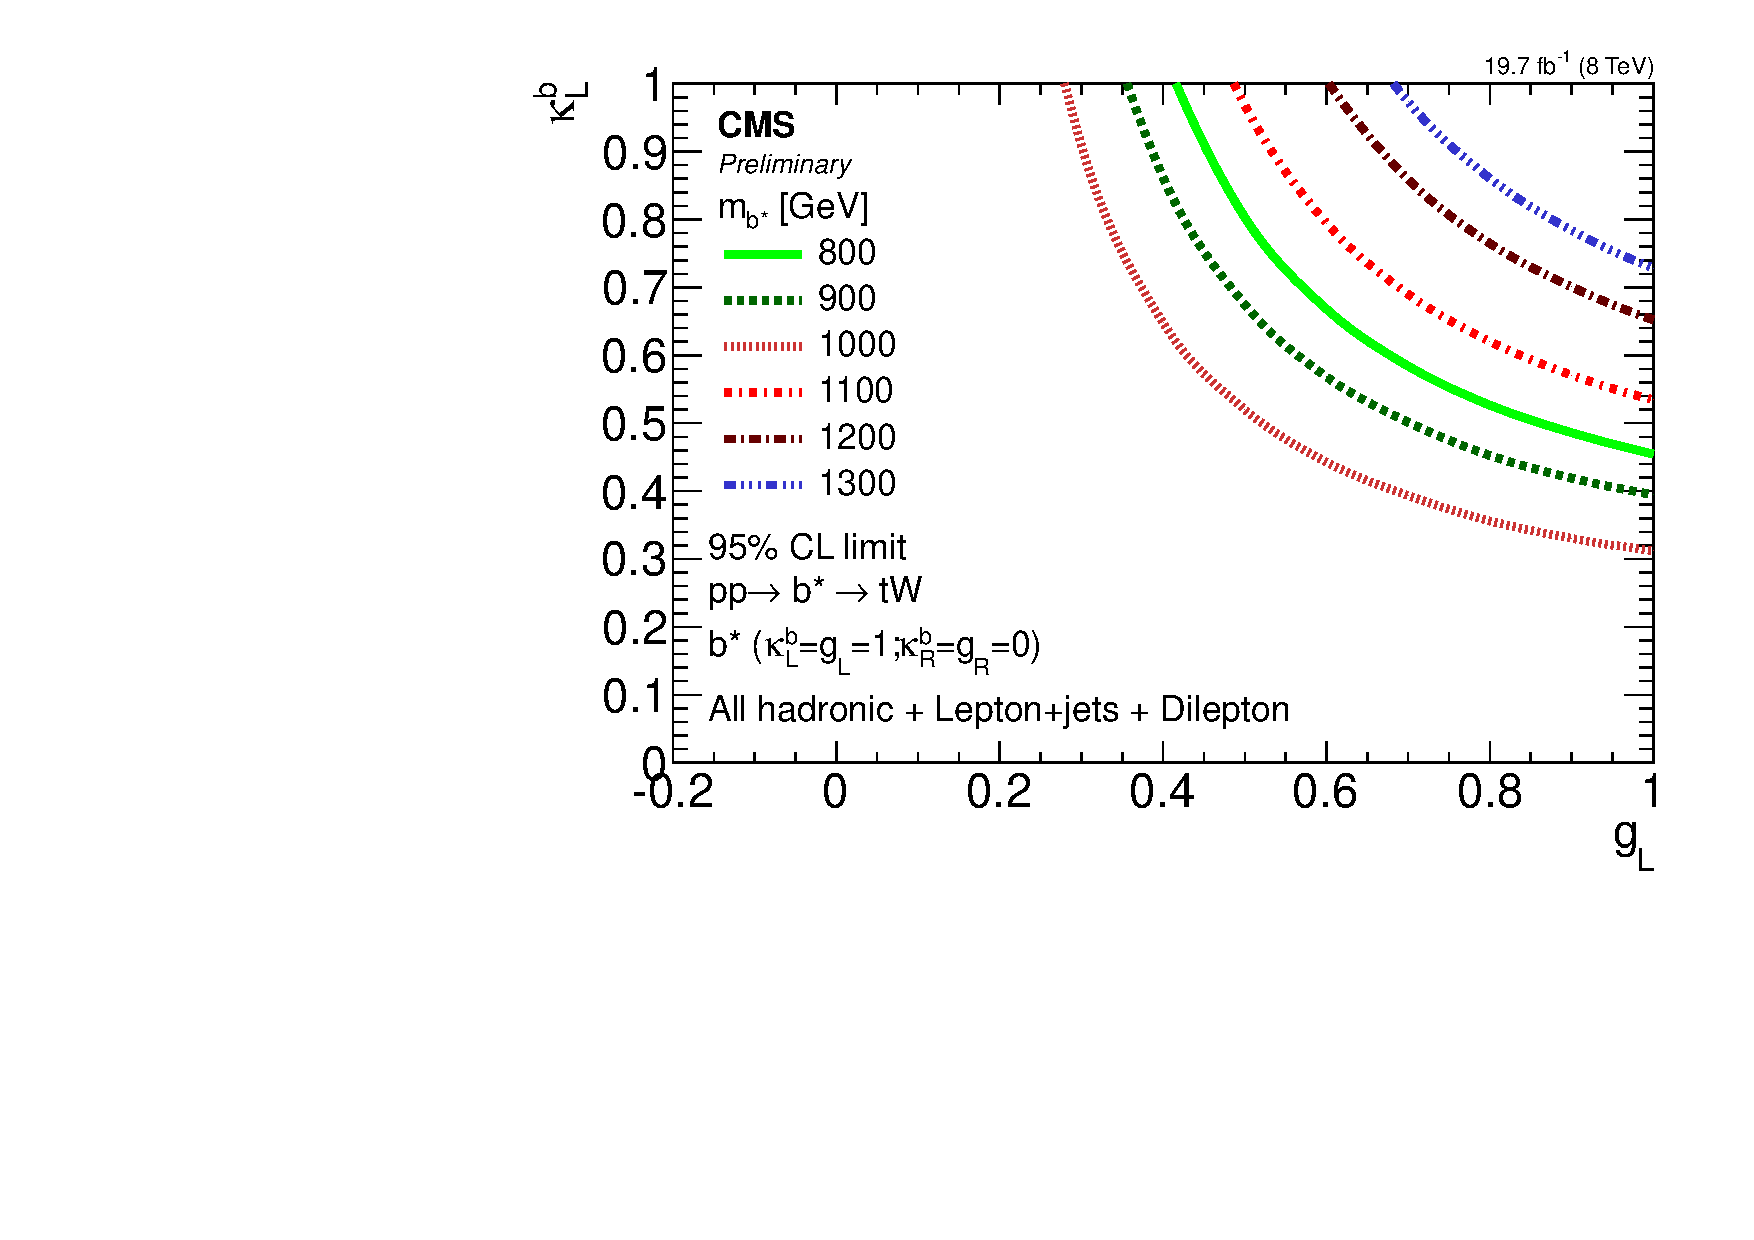
\includegraphics[width=0.6\textwidth]{AN-14-049/figs/bayesian_observed_hadronic_semileptonic_left_2Dlimit_plot.pdf}\\
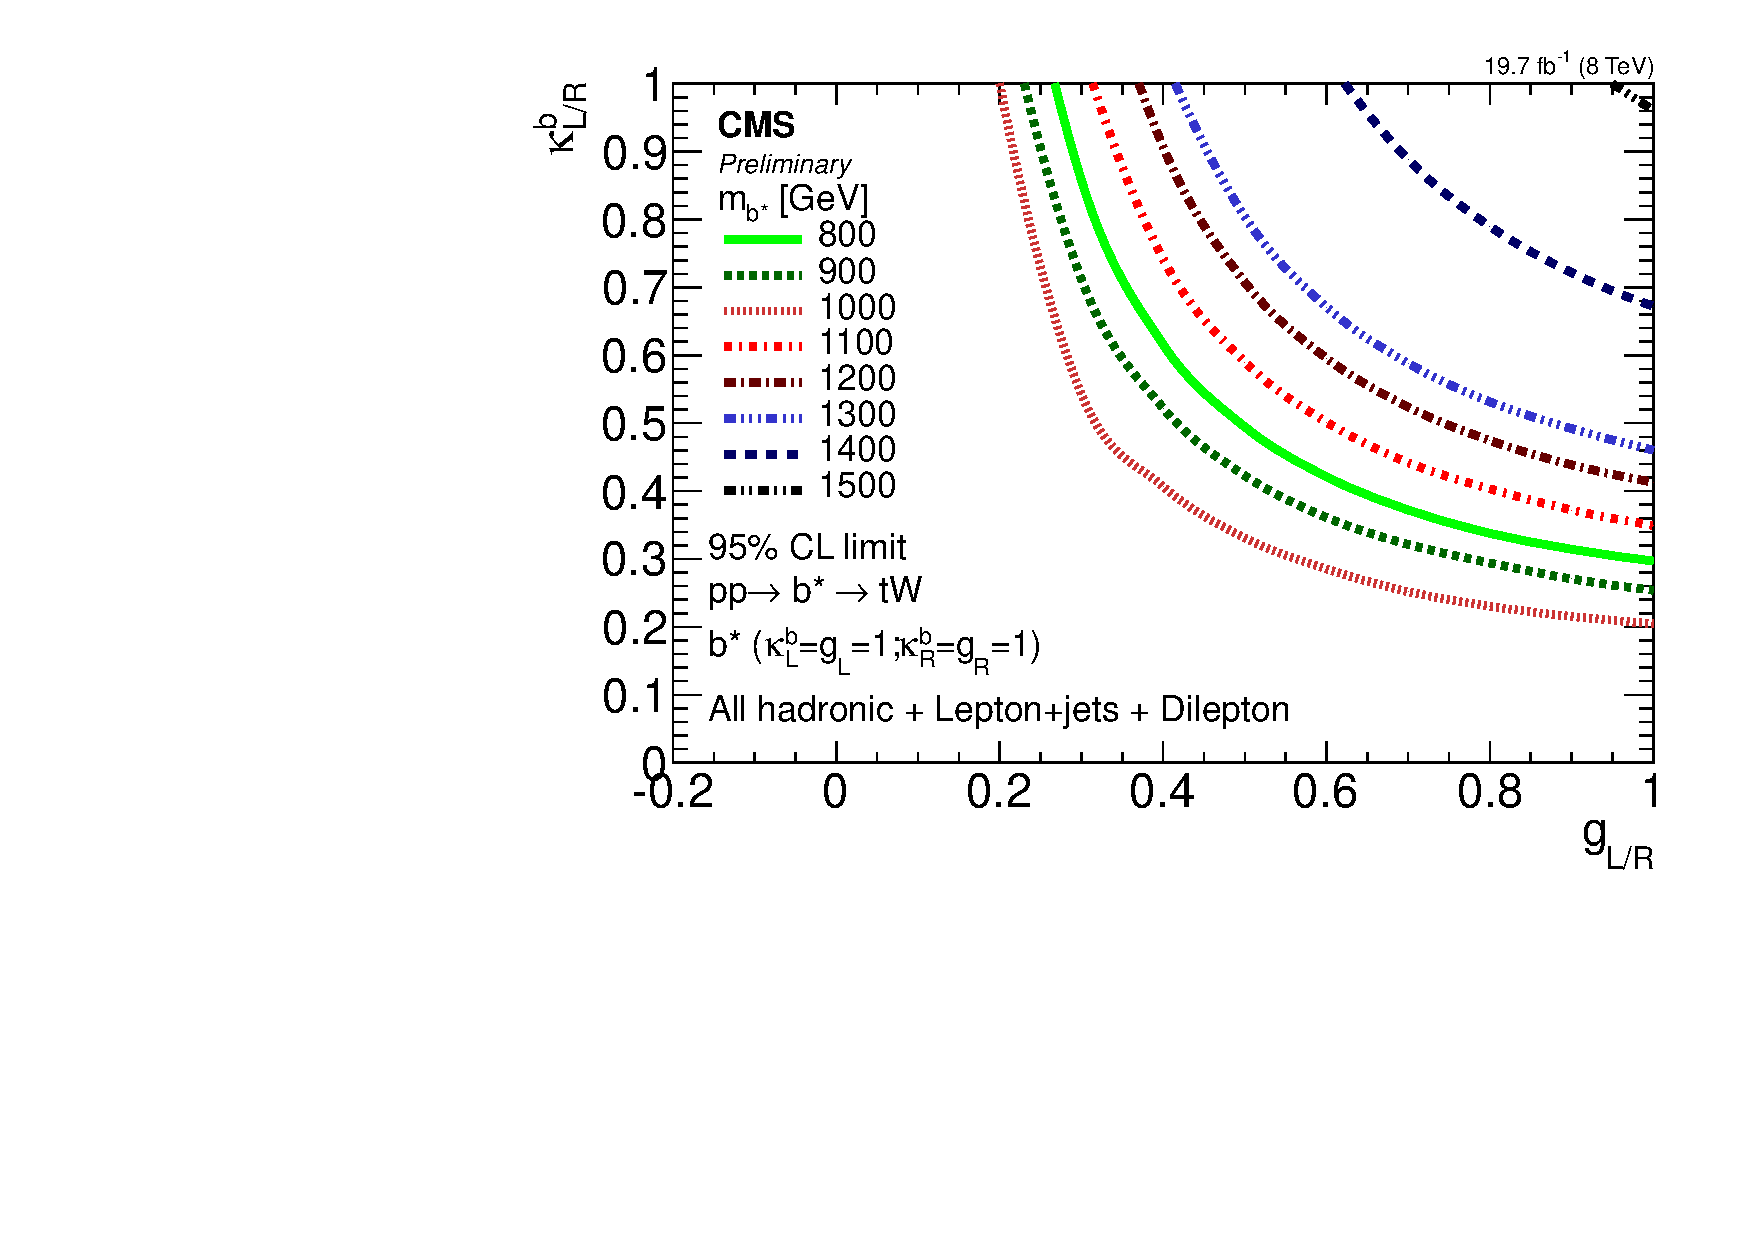
\includegraphics[width=0.6\textwidth]{AN-14-049/figs/bayesian_observed_hadronic_semileptonic_vector_2Dlimit_plot.pdf}\\
\caption{observed limit plot in the $\kappa$,$g$ plane.  The top, middle, and bottom plots show limits for right, left and vector-like coupling hypotheses respectively.}
\label{figs:bsthetalimit2dobs}
\end{figure}

\begin{figure}[htcb]
\centering
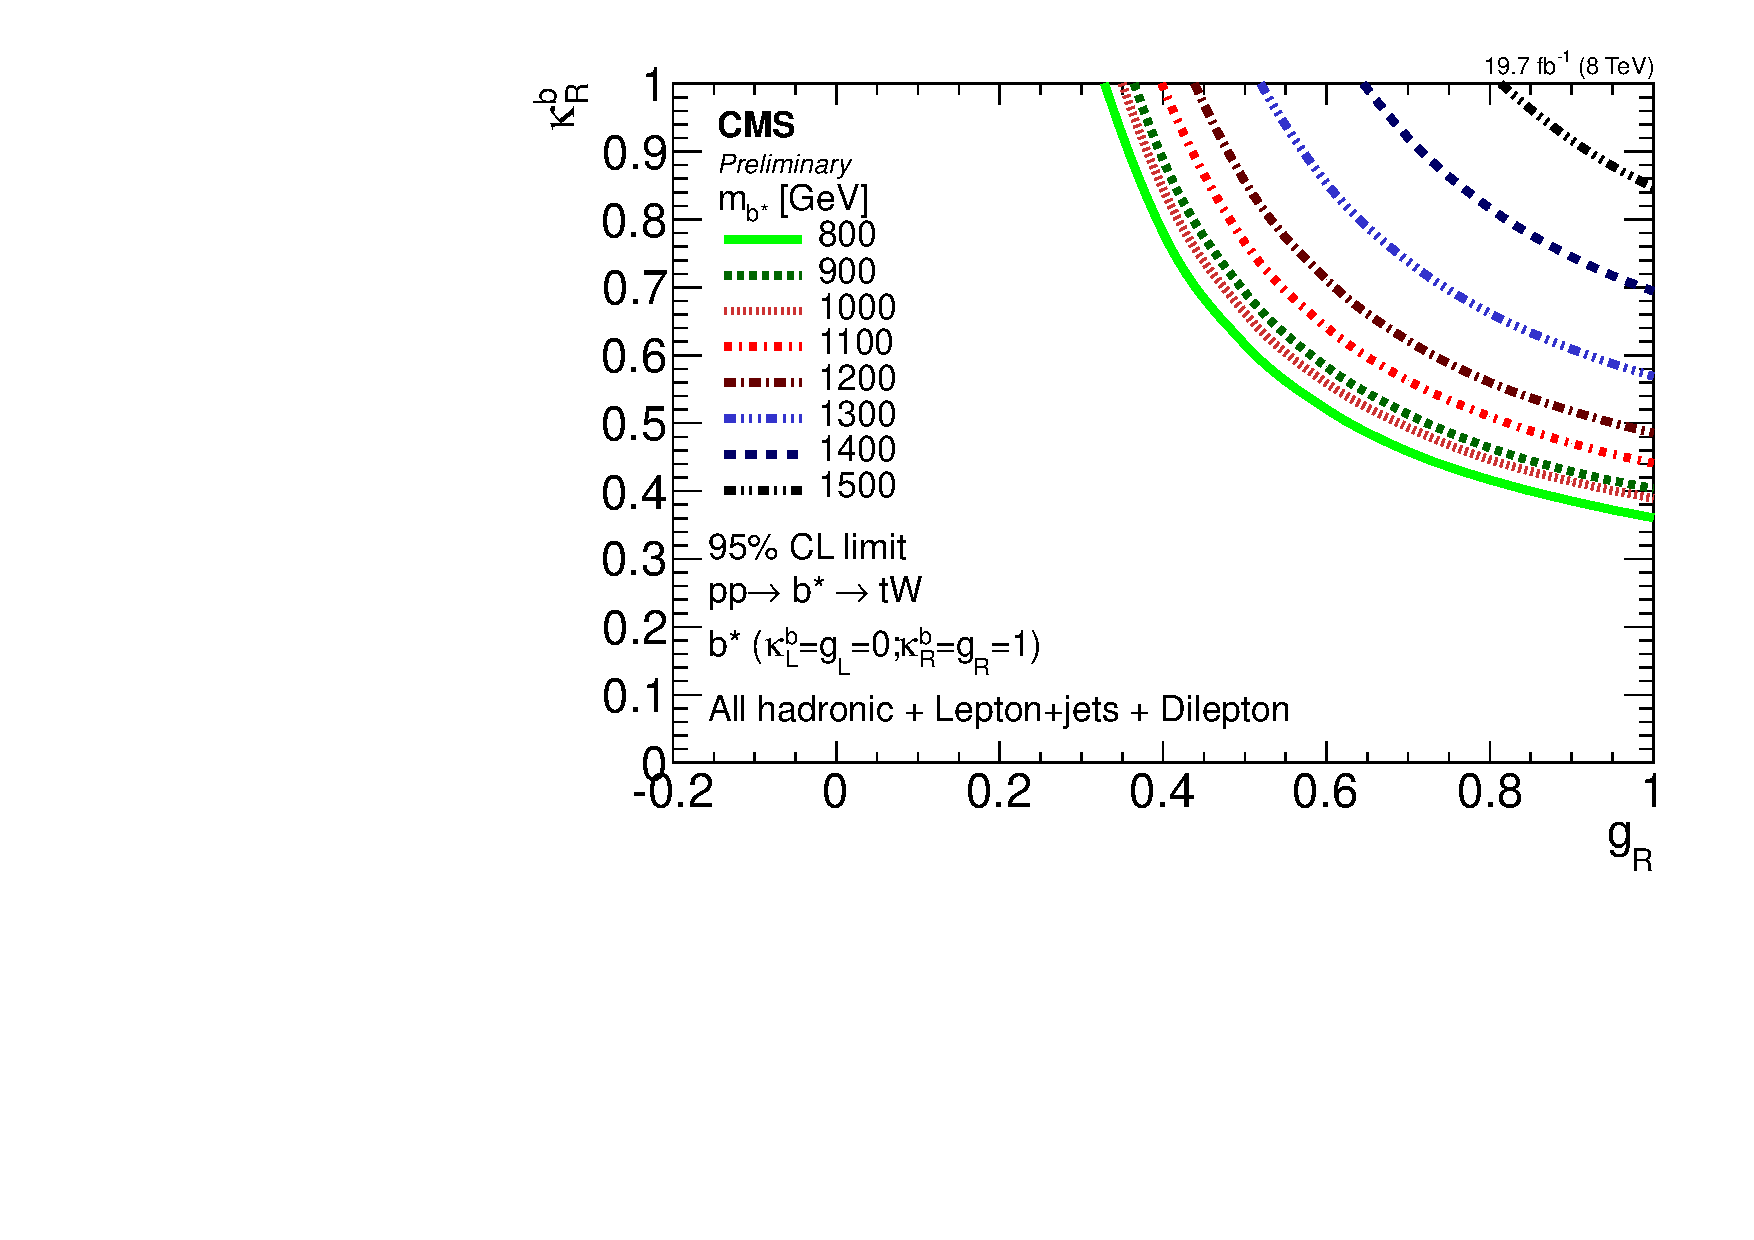
\includegraphics[width=0.6\textwidth]{AN-14-049/figs/bayesian_expected_hadronic_semileptonic_right_2Dlimit_plot.pdf}\\
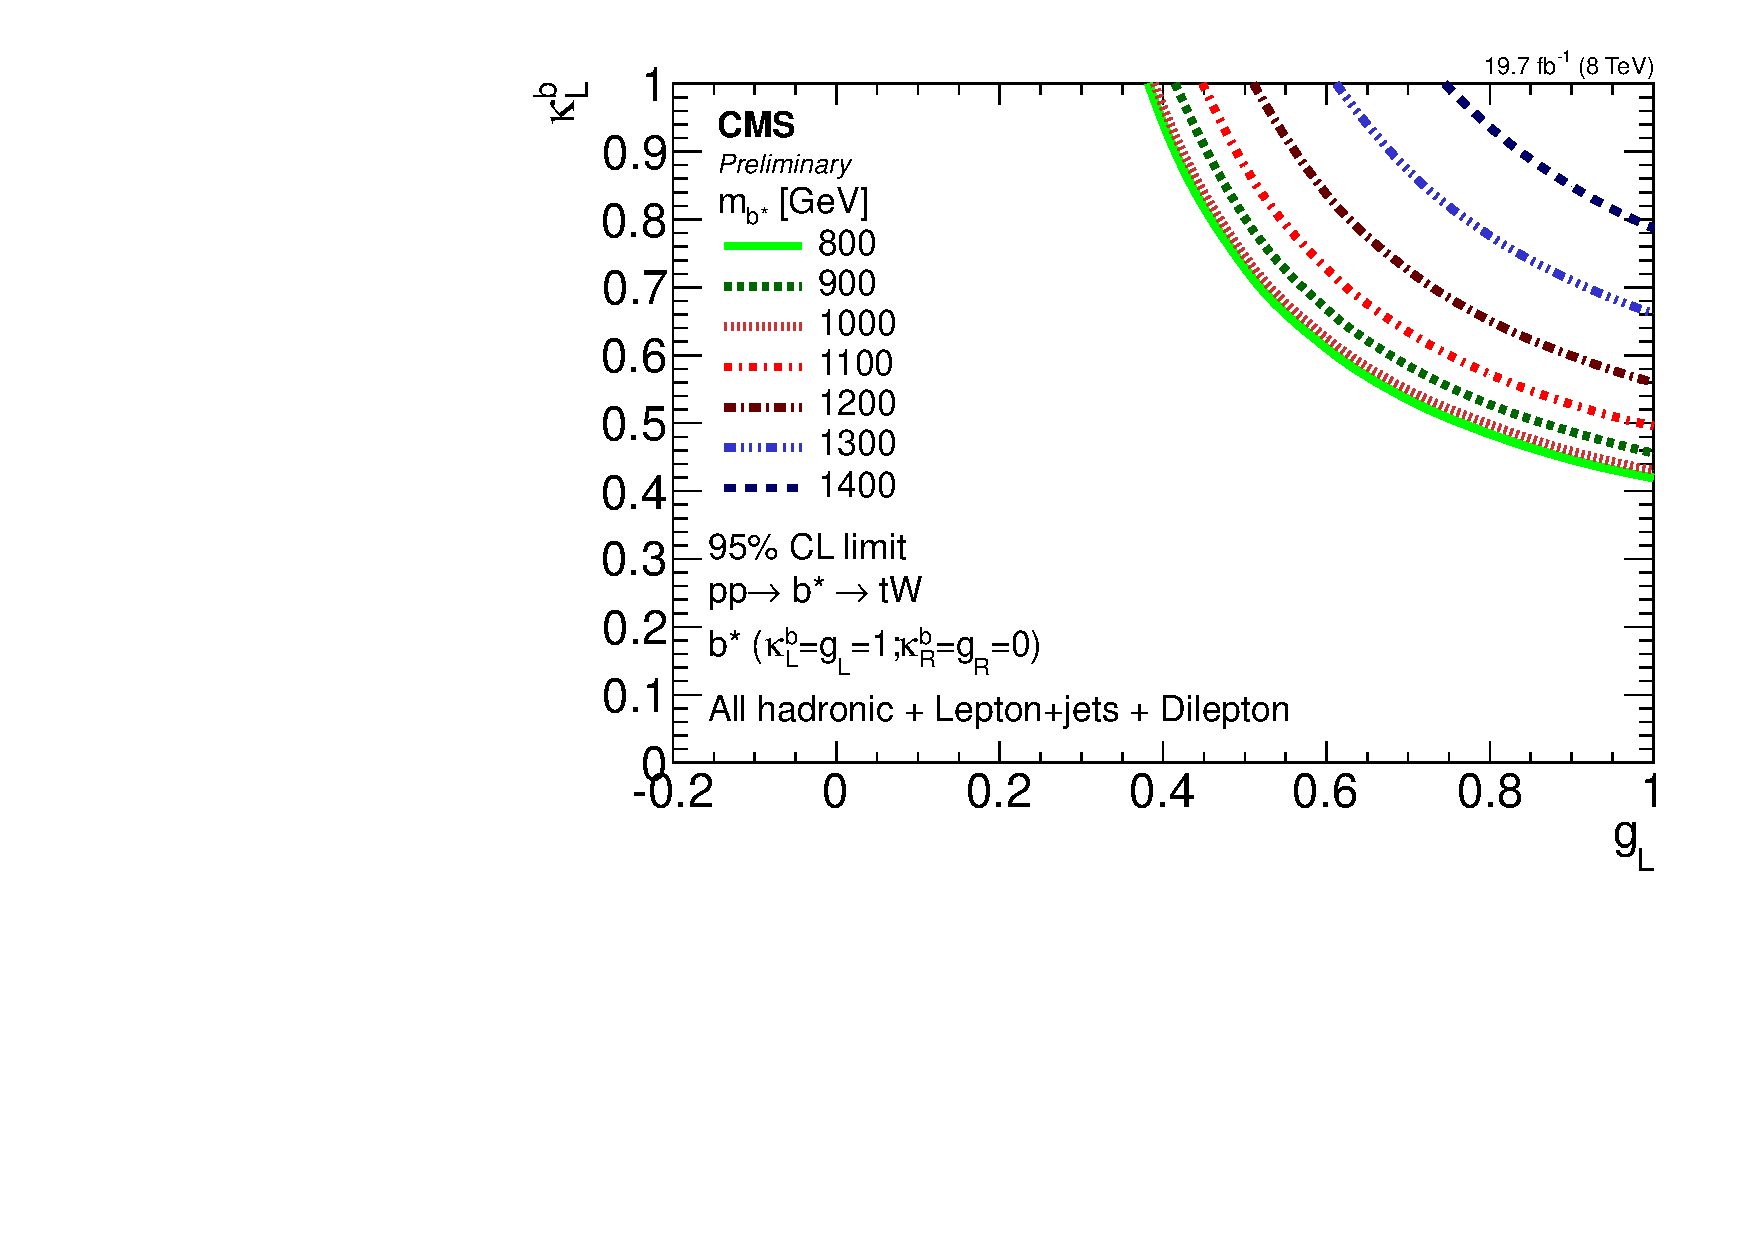
\includegraphics[width=0.6\textwidth]{AN-14-049/figs/bayesian_expected_hadronic_semileptonic_left_2Dlimit_plot.pdf}\\
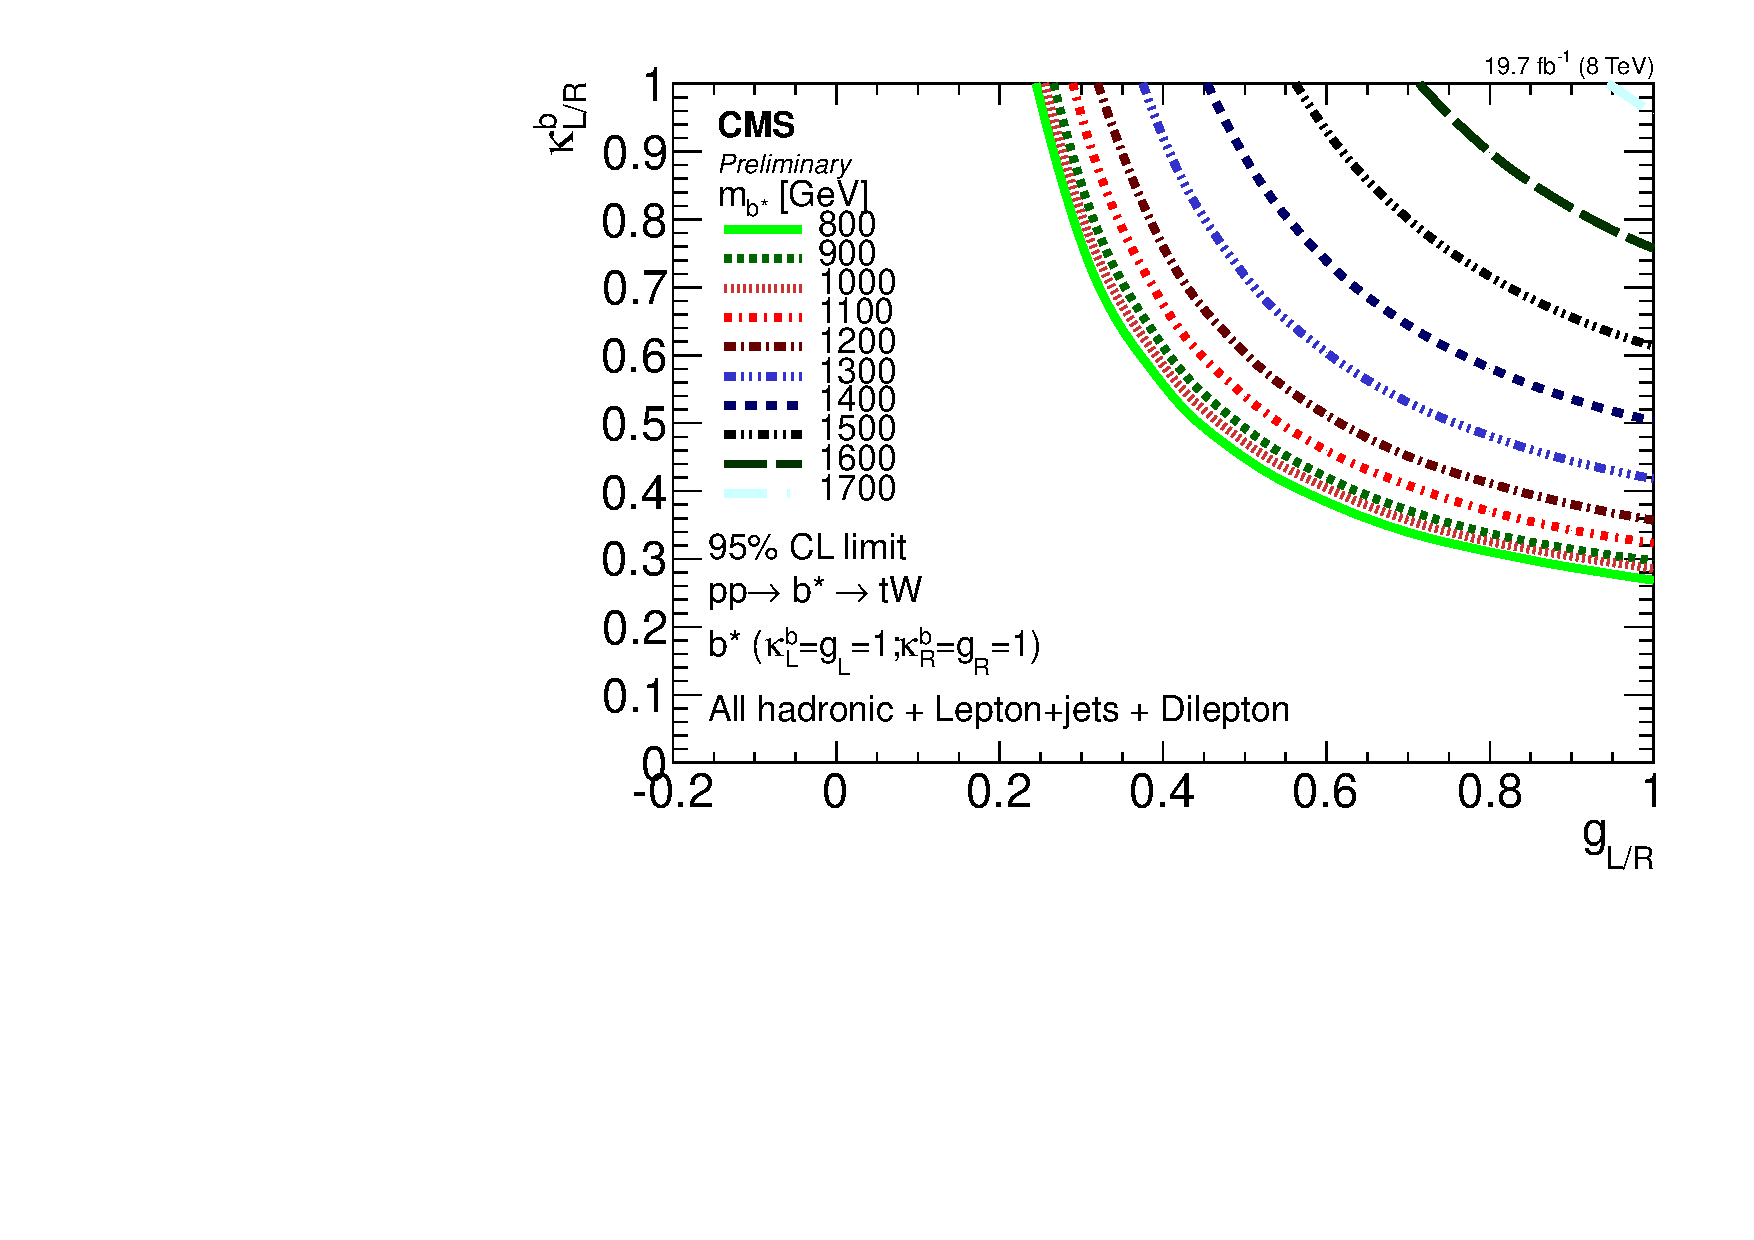
\includegraphics[width=0.6\textwidth]{AN-14-049/figs/bayesian_expected_hadronic_semileptonic_vector_2Dlimit_plot.pdf}\\
\caption{expected limit plot in the $\kappa$,$g$ plane.  The top, middle, and bottom plots show limits for right, left and vector-like coupling hypotheses respectively.}
\label{figs:bsthetalimit2dexp}
\end{figure}


\begin{sidewaysfigure}[htcb]
\centering
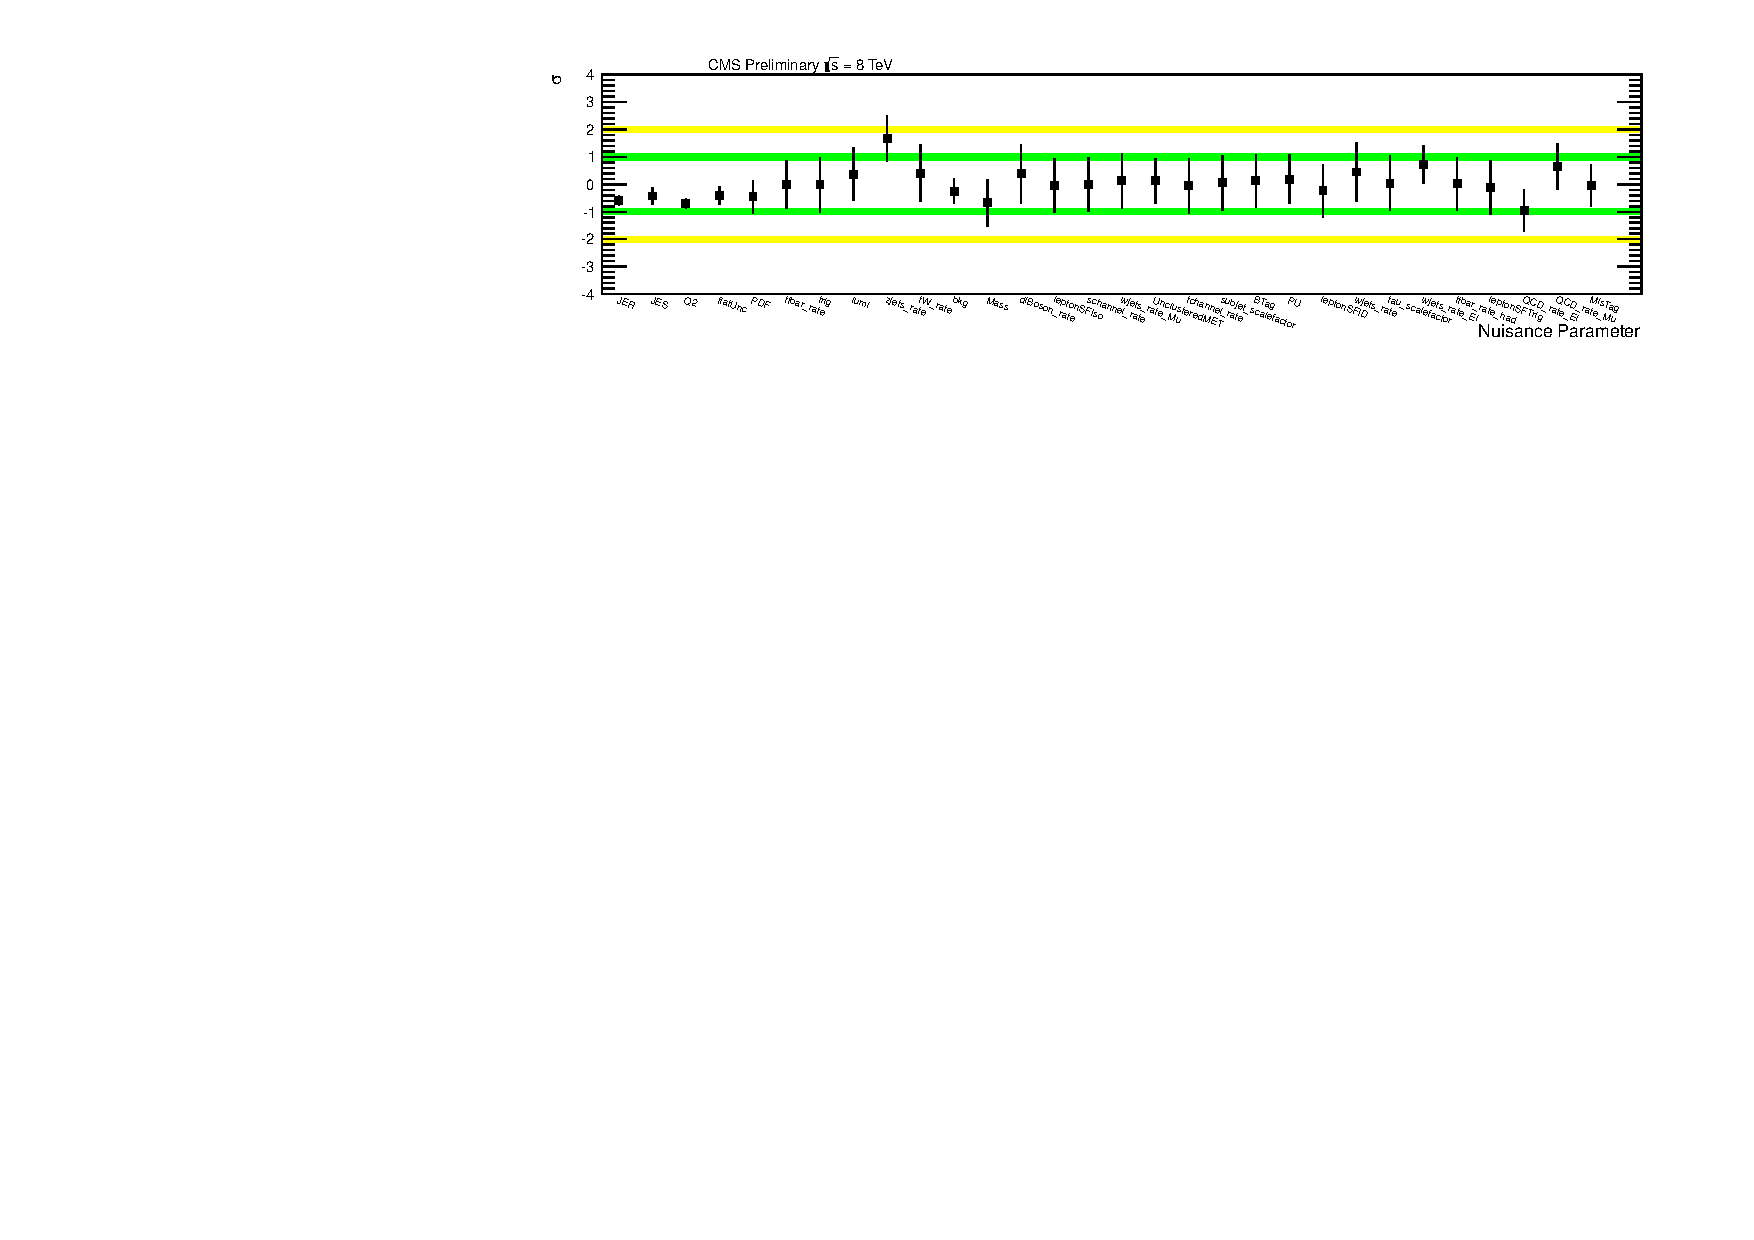
\includegraphics[width=1.0\textwidth]{AN-14-049/figs/nuisancerightbs1200.pdf}\\
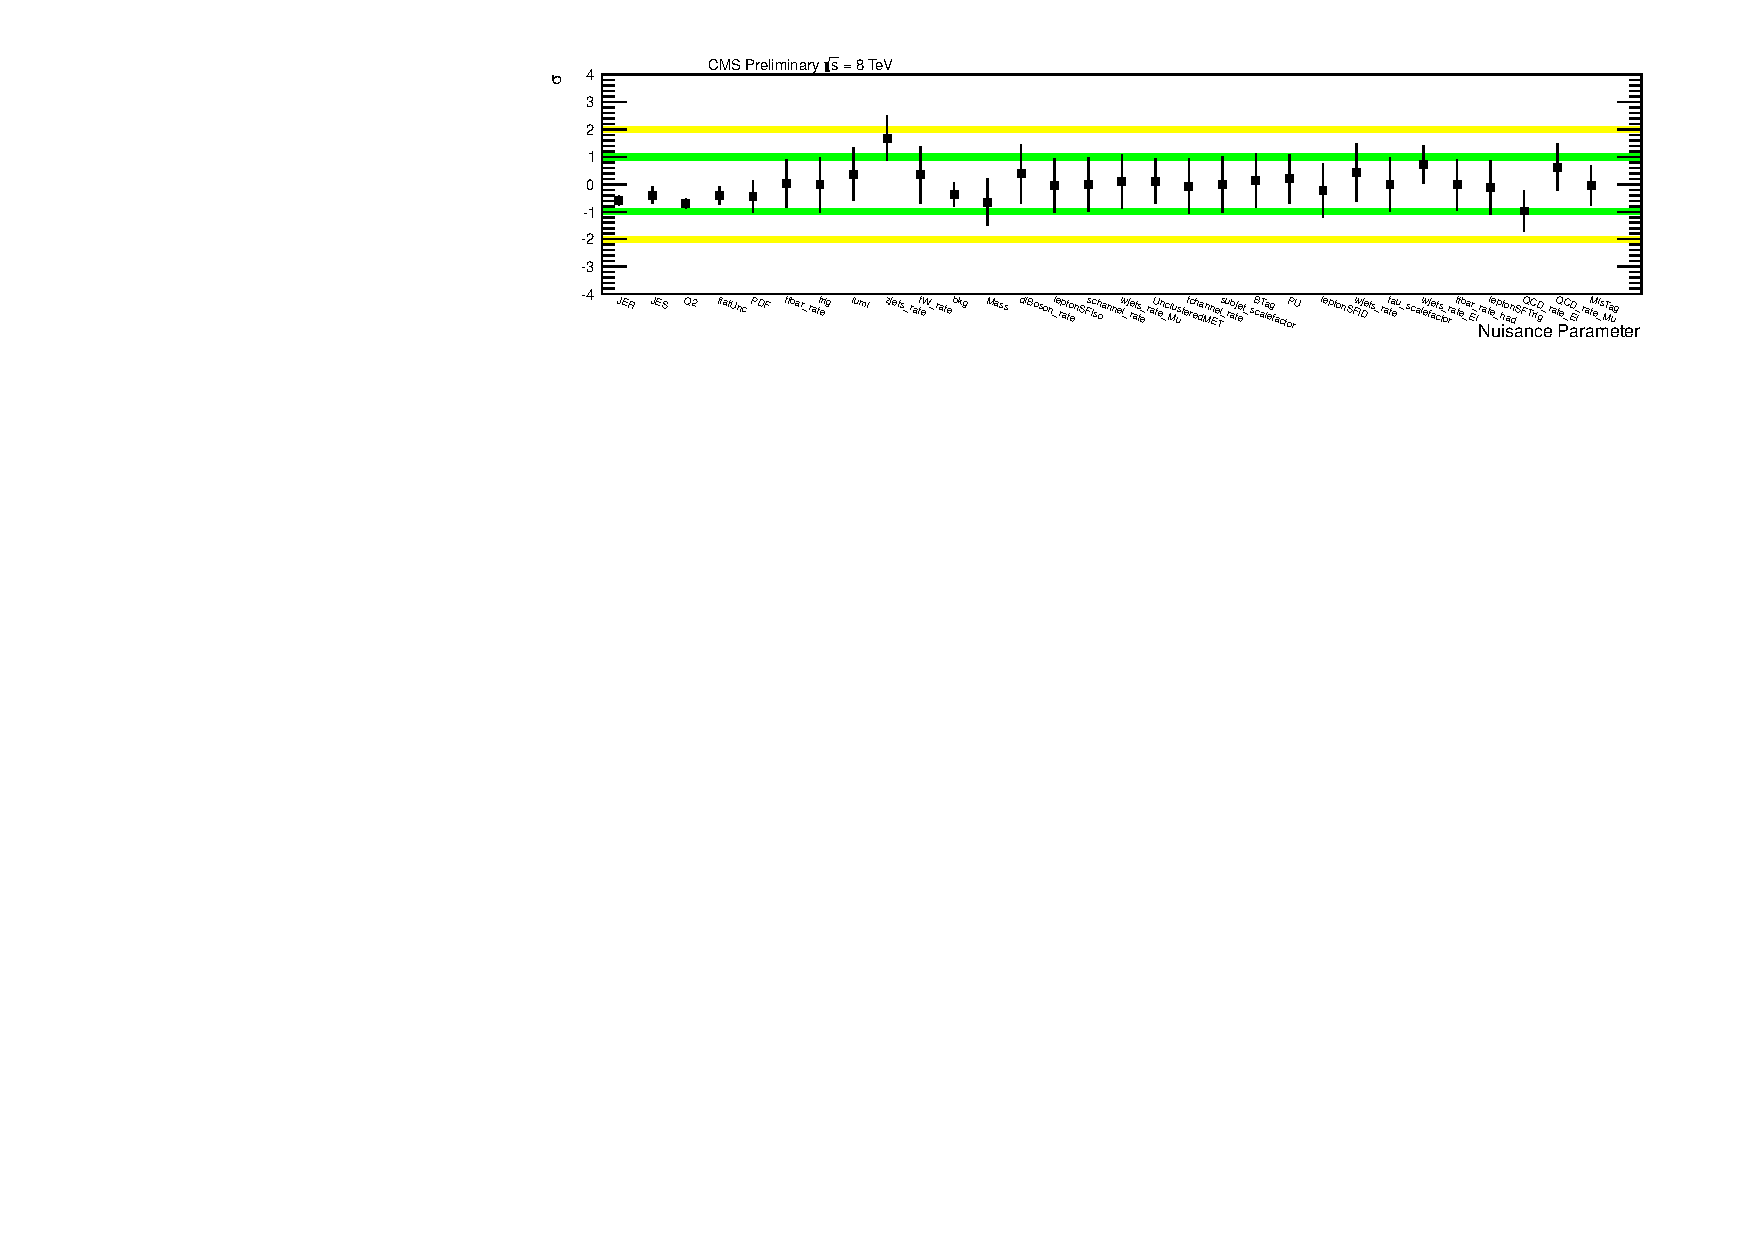
\includegraphics[width=1.0\textwidth]{AN-14-049/figs/nuisancerightbs1400.pdf}\\
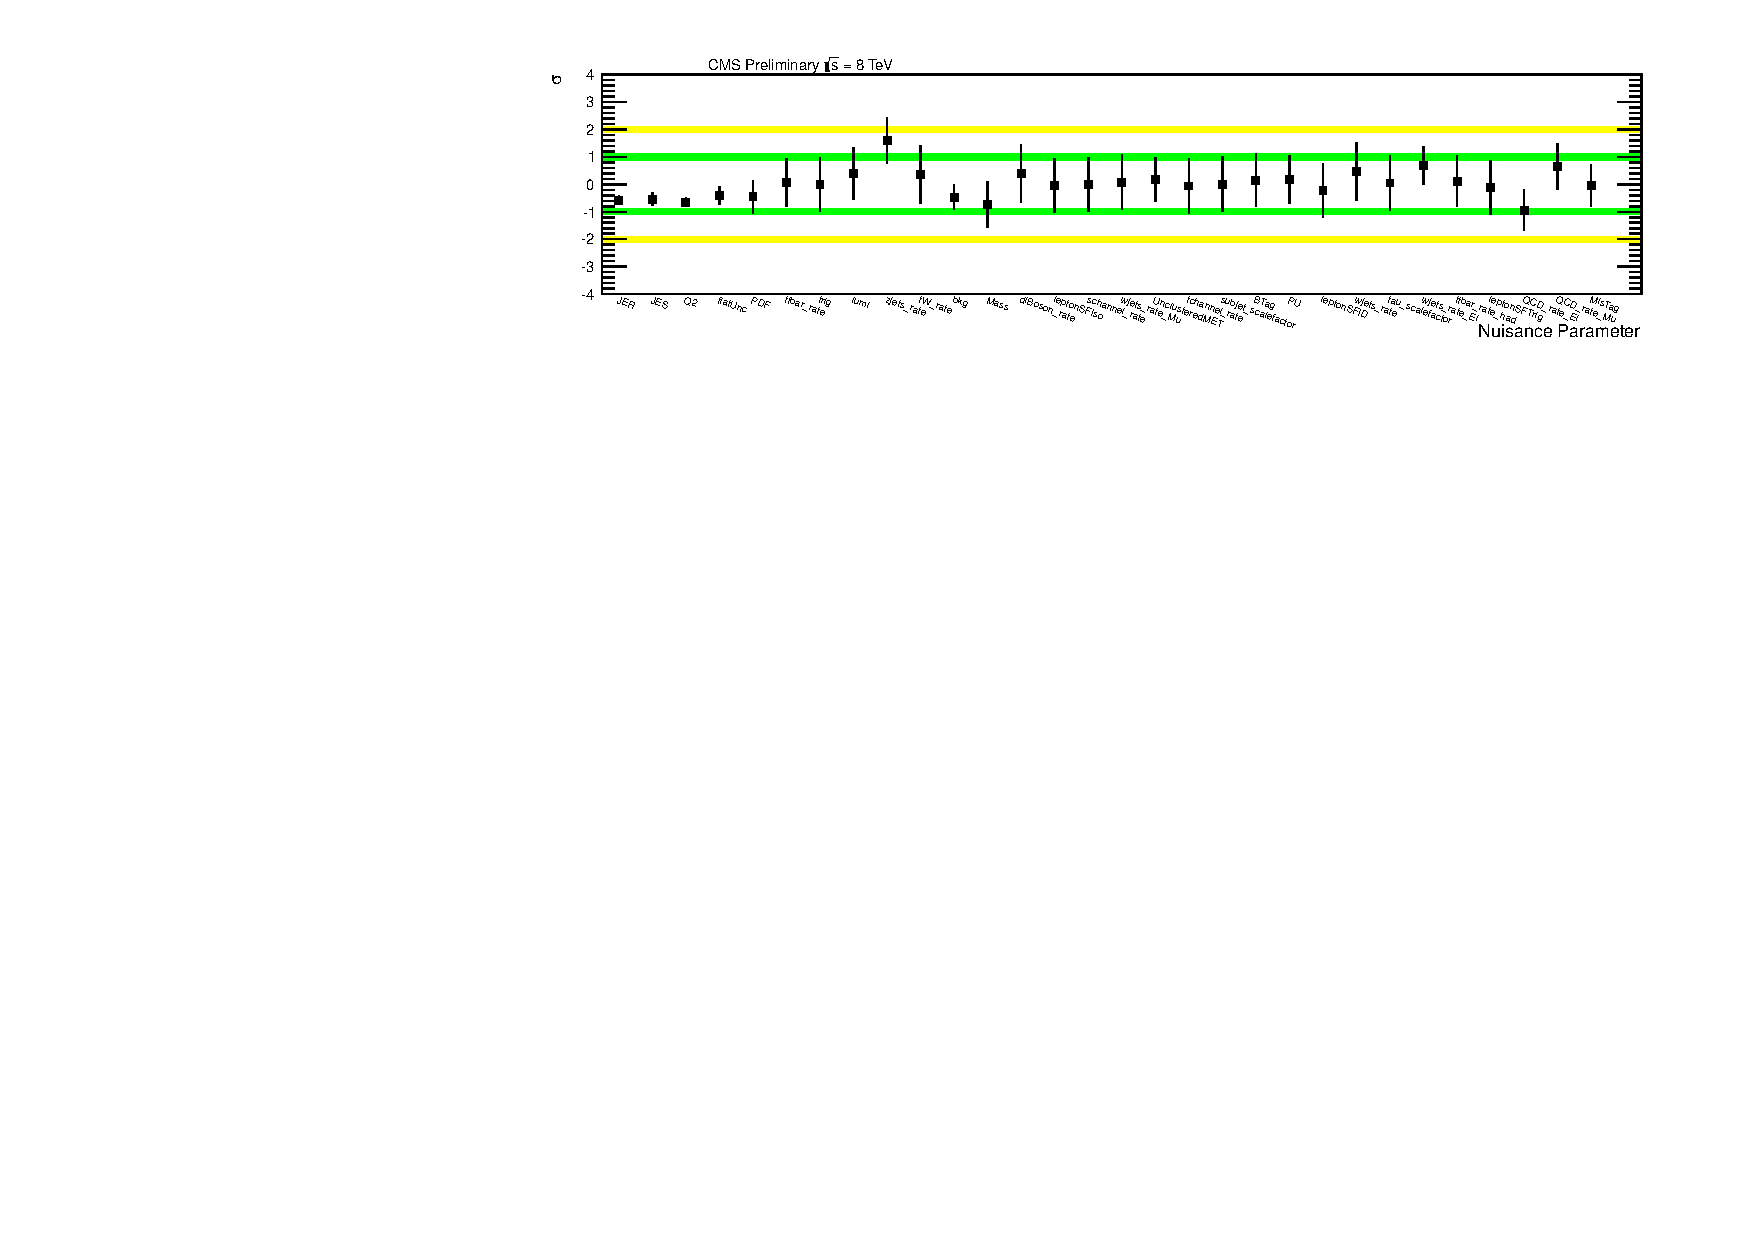
\includegraphics[width=1.0\textwidth]{AN-14-049/figs/nuisancerightbs1600.pdf}\\
\caption{Nuisance parameters after the Theta fit.  The Signal mass points here are 1200, 1400, and 1600 $\GeV$ for the top, middle, and bottom plots respectively.}
\label{figs:bsnuisance}
\end{sidewaysfigure}

\clearpage

\begin{table}[htcb]
\begin{center}
\bf{$\bs_{R}$ Cross-Section Upper Limits}\\
\begin{tabular}{c||c|c|c|c}
\hline\hline
\bf{$\mathrm{M_{\bs}}$} & \bf{observed}  & \bf{expected} & \bf{expected 1$\sigma$}  & \bf{expected 2$\sigma$} \\
\hline
\hline
800 & 0.490 & 0.492 & 0.335,0.723 & 0.243,1.039\\ 
900 & 0.188 & 0.303 & 0.202,0.446 & 0.140,0.611\\ 
1000 & 0.070 & 0.141 & 0.097,0.203 & 0.070,0.279\\ 
1100 & 0.103 & 0.096 & 0.068,0.138 & 0.050,0.186\\ 
1200 & 0.074 & 0.063 & 0.044,0.092 & 0.032,0.129\\ 
1300 & 0.052 & 0.045 & 0.032,0.067 & 0.023,0.098\\ 
1400 & 0.063 & 0.038 & 0.027,0.053 & 0.020,0.076\\ 
1500 & 0.067 & 0.030 & 0.021,0.043 & 0.015,0.061\\
1600 & 0.056 & 0.025 & 0.018,0.037 & 0.012,0.052\\ 
1700 & 0.037 & 0.023 & 0.016,0.034 & 0.011,0.049\\ 
1800 & 0.023 & 0.021 & 0.014,0.030 & 0.010,0.044\\ 
1900 & 0.021 & 0.020 & 0.014,0.030 & 0.010,0.042\\ 
2000 & 0.021 & 0.020 & 0.013,0.030 & 0.010,0.043\\ 
\hline
\end{tabular}
\end{center}
\caption{$\bs_R$ cross-section upper limits for given $\bs_R$ mass values.  Cross-section is in units of pb.}
\label{table:bsupperxsecR}
\end{table}



\begin{table}[htcb]
\begin{center}
\bf{$\bs_{L}$ Cross-Section Upper Limits}\\
\begin{tabular}{c||c|c|c|c}
\hline\hline
\bf{$\mathrm{M_{\bs}}$} & \bf{observed}  & \bf{expected} & \bf{expected 1$\sigma$}  & \bf{expected 2$\sigma$} \\
\hline
\hline
800 & 0.617 & 0.666 & 0.454,0.984 & 0.344,1.366\\ 
900 & 0.236 & 0.387 & 0.258,0.571 & 0.172,0.782\\ 
1000 & 0.086 & 0.173 & 0.119,0.251 & 0.087,0.337\\ 
1100 & 0.123 & 0.119 & 0.085,0.174 & 0.063,0.236\\ 
1200 & 0.097 & 0.083 & 0.057,0.120 & 0.042,0.173\\ 
1300 & 0.068 & 0.059 & 0.042,0.088 & 0.030,0.127\\ 
1400 & 0.074 & 0.048 & 0.033,0.067 & 0.025,0.096\\ 
1500 & 0.088 & 0.040 & 0.028,0.057 & 0.020,0.082\\
1600 & 0.077 & 0.034 & 0.023,0.049 & 0.016,0.068\\ 
1700 & 0.049 & 0.030 & 0.021,0.044 & 0.014,0.062\\ 
1800 & 0.032 & 0.028 & 0.019,0.040 & 0.013,0.059\\ 
1900 & 0.031 & 0.027 & 0.018,0.039 & 0.013,0.057\\ 
2000 & 0.032 & 0.027 & 0.018,0.040 & 0.014,0.060\\ 
\hline
\end{tabular}
\end{center}
\caption{$\bs_L$ cross-section upper limits for given $\bs_L$ mass values.  Cross-section is in units of pb.}
\label{table:bsupperxsecL}
\end{table}



\begin{table}[htcb]
\begin{center}
\bf{$\bs_{LR}$ Cross-Section Upper Limits}\\
\begin{tabular}{c||c|c|c|c}
\hline\hline
\bf{$\mathrm{M_{\bs}}$} & \bf{observed}  & \bf{expected} & \bf{expected 1$\sigma$}  & \bf{expected 2$\sigma$} \\
\hline
\hline
800 & 0.510 & 0.570 & 0.384,0.840 & 0.285,1.137\\ 
900 & 0.208 & 0.337 & 0.226,0.496 & 0.157,0.686\\ 
1000 & 0.080 & 0.156 & 0.107,0.220 & 0.079,0.313\\ 
1100 & 0.112 & 0.107 & 0.074,0.152 & 0.057,0.210\\ 
1200 & 0.084 & 0.072 & 0.050,0.104 & 0.035,0.146\\ 
1300 & 0.058 & 0.051 & 0.036,0.076 & 0.026,0.108\\ 
1400 & 0.064 & 0.042 & 0.030,0.059 & 0.022,0.085\\ 
1500 & 0.074 & 0.034 & 0.024,0.050 & 0.018,0.072\\
1600 & 0.067 & 0.029 & 0.020,0.042 & 0.014,0.060\\ 
1700 & 0.041 & 0.026 & 0.018,0.038 & 0.013,0.054\\ 
1800 & 0.027 & 0.024 & 0.016,0.035 & 0.011,0.050\\ 
1900 & 0.025 & 0.023 & 0.016,0.033 & 0.011,0.050\\ 
2000 & 0.024 & 0.023 & 0.015,0.033 & 0.012,0.050\\ 
\hline
\end{tabular}
\end{center}
\caption{$\bs_LR$ cross-section upper limits for given $\bs_{LR}$ mass values.  Cross-section is in units of pb.}
\label{table:bsupperxsecLR}
\end{table}


\begin{table}[hp]
\centering
\begin{tabular}{r||r|r|r}
\hline
&left-handed&right-handed&vector like\\
\hline\hline
\multicolumn{4}{c}{Lepton + jets, dilepton and full hadronic channel combined} \\
\hline
expected 95\% CL limit [GeV] &  1500 & 1580 & 1730 \\
observed 95\% CL limit [GeV] &  1390 & 1420 & 1520 \\
\hline
\multicolumn{4}{c}{Full hadronic channel only} \\
\hline
expected 95\% CL limit [GeV] & 890 - 1480 & 880 - 1550 & 820 - 1700 \\
observed 95\% CL limit [GeV] & 880 - 1390 & 820 - 1430 & 1530 \\
\hline
\multicolumn{4}{c}{Lepton + jets channel only} \\
\hline
expected 95\% CL limit [GeV] & 940  & 990  & 1130 \\
observed 95\% CL limit [GeV] & 1030 & 1070 & 1170 \\
\hline
\multicolumn{4}{c}{Dilepton channel only} \\
\hline
expected 95\% CL limit [GeV] & 1060 & 1100 & 1210 \\
observed 95\% CL limit [GeV] & 1020 & 1050 & 1160 \\
\hline
\end{tabular}
\caption{95\% CLs limit for the left-, right-handed and vector like excited bottom quark in the full hadronic, lepton+jets and dilepton channel combined and separately at the benchmark point of unit couplings.}
\label{limitTable}
\end{table}


%\begin{sidewaystable}[htcb]
%\begin{center}
%\begin{small}
%\resizebox{0.5\textwidth}{!}\begin{tabular}{c||ccccccccccccccccccccccccccccccc}
%\multicolumn{7}{c}{Nuisance parameters} \\
%\hline\hline 
%Sample & Q2 & trig & diBoson_rate & leptonSFIso & schannel_rate & flatUnc & tchannel_rate & BTag & PU & leptonSFID & wjets_rate & wjets_rate_El & leptonSFTrig & JER & JES & bkg & wjets_rate_Mu & ttbar_rate & zjets_rate & beta_signal & Q2_slep & Mass & MisTag & lumi & PDF & UnclusteredMET & subjet_scalefactor & reweight & Matching & ttbar_rate_had & tau_scalefactor & QCD_rate_El & QCD_rate_Mu & tW_rate \\
%\hline
%bs1700 & -0.468874370984 \pm 0.627981899378 & -0.0122371561786 \pm 0.993800943621 & 0.115192917453 \pm 1.00993607365 & -0.105487521352 \pm 1.00397595182 & 0.00708062176357 \pm 0.994787272412 & -0.0150442089712 \pm 0.385115784756 & 0.0442891145828 \pm 0.998622797741 & -0.129760603569 \pm 1.02796946164 & 0.407341679805 \pm 0.926671522598 & -0.545651575436 \pm 0.971204990917 & 0.499766026154 \pm 1.05826770381 & 1.24382124204 \pm 0.854974821264 & -0.324766261624 \pm 1.00137381842 & -0.226531018641 \pm 0.338393044899 & -0.95818742926 \pm 0.239713682488 & -0.554744255865 \pm 0.616365912328 & -0.434931233537 \pm 0.938368509922 & -0.932142353982 \pm 0.971440752775 & 0.0142302841684 \pm 0.892948457579 & 1.65401238303 \pm 1.03664914077 & -0.351439331927 \pm 0.203115380201 & -0.536833395528 \pm 0.789297102738 & 0.0114323425774 \pm 1.04303980927 & -0.352076777363 \pm 0.993054831933 & 0.0618805590836 \pm 1.10397736912 & 0.00952669776658 \pm 0.567037046274 & 0.332917544798 \pm 1.02546156753 & 0.926671510852 \pm 0.247643188535 & -0.356006227546 \pm 0.256856832238 & 0.209983073242 \pm 0.990923684302 & 0.282440811301 \pm 0.998169555272 & 0.239836656613 \pm 1.02489406944 & 0.0217627716757 \pm 0.996957562863 & 0.304555961003 \pm 1.08187835857 \\
%\hline
%bs1800 & -0.77633953053 \pm 0.56087310659 & -0.0143976257406 \pm 0.993802502601 & 0.196102952444 \pm 1.0270476453 & -0.105790458404 \pm 1.00484341652 & 0.00665770334836 \pm 0.994711979744 & -0.156266394091 \pm 0.352052716331 & 0.0395338110348 \pm 0.996152977166 & 0.00258593834482 \pm 0.939620829284 & 0.364467078669 \pm 0.931863368393 & -0.573930457305 \pm 0.962422511563 & 0.453243834195 \pm 1.0576717188 & 1.46621636005 \pm 0.758963247138 & -0.333194592109 \pm 0.994150523436 & -0.260191141622 \pm 0.311057983599 & -0.640849304115 \pm 0.328445736297 & -0.43509565588 \pm 0.634976056899 & -0.471187489693 \pm 0.852227291456 & -0.715201870223 \pm 0.903668004119 & 0.205394687448 \pm 0.880880750445 & 0.326939697529 \pm 1.08455001343 & -0.317452212074 \pm 0.223059177721 & -0.64487801072 \pm 0.834630090889 & 0.0180228890222 \pm 1.00991355855 & -0.209273220535 \pm 0.969341937258 & 0.254533028582 \pm 0.669960920161 & -0.0640267894157 \pm 0.58914522845 & 0.269595190187 \pm 1.0224697774 & 0.942066579198 \pm 0.25029663609 & 0.312408379756 \pm 0.318751262061 & 0.392277768694 \pm 0.984722663149 & 0.307550584941 \pm 0.995079507806 & 0.245537879125 \pm 1.02328350407 & 0.0121138782106 \pm 0.995468336819 & 0.349304296572 \pm 1.06340610358 \\
%\hline
%bs1300 & -0.843111026561 \pm 0.539007709647 & -0.0141473093488 \pm 0.993805425765 & 0.189599308391 \pm 1.02501046275 & -0.105150313439 \pm 1.00487615224 & 0.00653022670322 \pm 0.994654205472 & -0.156644652172 \pm 0.350602721701 & 0.0360442711789 \pm 0.995849885334 & 0.00195983001504 \pm 0.939829795843 & 0.358557643214 \pm 0.930723900816 & -0.570753330354 \pm 0.962301764143 & 0.449497033064 \pm 1.05683960245 & 1.46115004808 \pm 0.757180782195 & -0.330567000973 \pm 0.994113193487 & -0.280456126251 \pm 0.308332691502 & -0.622898606618 \pm 0.309792871379 & -0.413273147382 \pm 0.609882231884 & -0.481578057555 \pm 0.851888643701 & -0.707478671973 \pm 0.902516878099 & 0.21113434379 \pm 0.882755845525 & 0.0775231619629 \pm 0.190392410391 & -0.311223553041 \pm 0.221908499188 & -0.63939202782 \pm 0.82970322419 & 0.0150905609596 \pm 1.01586772343 & -0.195583379221 \pm 0.968563342576 & 0.254568297202 \pm 0.664137438749 & -0.066738129845 \pm 0.589291367478 & 0.242495333859 \pm 1.02868378899 & 0.943631515609 \pm 0.251014660211 & 0.318214816367 \pm 0.306398293533 & 0.327679227241 \pm 1.00070147817 & 0.268099697762 \pm 1.00492023999 & 0.244332404196 \pm 1.02283529252 & 0.0113034514017 \pm 0.995342752352 & 0.326509028772 \pm 1.05907959476 \\
%\hline
%bs1400 & -0.895594259033 \pm 0.531888762625 & -0.0125821103906 \pm 0.993799761266 & 0.194454407536 \pm 1.02542545961 & -0.103068673869 \pm 1.00473806092 & 0.00624787364162 \pm 0.994616425168 & -0.164804799508 \pm 0.348908165181 & 0.0280524659048 \pm 0.995287355421 & 0.0158030944024 \pm 0.940361261173 & 0.364378650282 \pm 0.929009873956 & -0.560207201163 \pm 0.962237287673 & 0.440802452637 \pm 1.05573858841 & 1.45603634985 \pm 0.757809064034 & -0.324543728903 \pm 0.994221737933 & -0.3086708493 \pm 0.301123647164 & -0.603790802486 \pm 0.29450164273 & -0.464790678819 \pm 0.59876381863 & -0.496611712371 \pm 0.853558045725 & -0.654917757359 \pm 0.89981201442 & 0.218982417146 \pm 0.887247653352 & 0.328174042104 \pm 0.287240741279 & -0.303357847601 \pm 0.220810730989 & -0.626499374175 \pm 0.819532762099 & 0.0105228329233 \pm 1.01980195933 & -0.190431113759 \pm 0.968255324927 & 0.229861726283 \pm 0.668857041289 & -0.0703660911238 \pm 0.587944927517 & 0.17425401416 \pm 1.02672180743 & 0.950109513239 \pm 0.25150772141 & 0.319008042915 \pm 0.304015562892 & 0.232875557883 \pm 0.980062051523 & 0.191868185039 \pm 1.00001115726 & 0.241974110577 \pm 1.02241512886 & 0.0107651385665 \pm 0.995260542188 & 0.25494671038 \pm 1.05430513735 \\
%\hline
%bs2000 & -0.799304378603 \pm 0.541645608004 & -0.0146262385664 \pm 0.99380093954 & 0.20631656961 \pm 1.02583277682 & -0.10570632749 \pm 1.00502760573 & 0.00673552681286 \pm 0.994671835161 & -0.162771875167 \pm 0.351398437494 & 0.0401997004607 \pm 0.996059857039 & 0.00191961411313 \pm 0.93998617892 & 0.36317024801 \pm 0.931570128282 & -0.575841647686 \pm 0.962170768975 & 0.451306886708 \pm 1.05728693061 & 1.46486315866 \pm 0.757617707434 & -0.334025375463 \pm 0.994070473594 & -0.258137116705 \pm 0.312770043199 & -0.626868372013 \pm 0.315350897737 & -0.419196199774 \pm 0.633655258464 & -0.472010951569 \pm 0.850784721606 & -0.70813300356 \pm 0.902647199377 & 0.210713023165 \pm 0.879852005518 & 0.405558174327 \pm 2.45289377051 & -0.317029535654 \pm 0.222790182968 & -0.64367274067 \pm 0.833683398183 & 0.0167087097181 \pm 1.01329088847 & -0.202349920687 \pm 0.968939259048 & 0.257044540192 \pm 0.66438580573 & -0.0654566381707 \pm 0.589233022172 & 0.263326863187 \pm 1.02120556869 & 0.942549125447 \pm 0.250683699245 & 0.316487862024 \pm 0.312452563901 & 0.411683857118 \pm 0.981946482759 & 0.310166346987 \pm 0.993840284025 & 0.245963545404 \pm 1.02296873679 & 0.0118563796647 \pm 0.99541657179 & 0.346754886698 \pm 1.0600704663 \\
%\hline
%bs1000 & 0.414856295355 \pm 0.740680923582 & -0.0157555985065 \pm 0.993810076387 & 0.188726330418 \pm 1.0197557723 & -0.106801243308 \pm 1.00497098824 & 0.00695645964683 \pm 0.994711964249 & -0.127859405509 \pm 0.350655778473 & 0.0397543716495 \pm 0.996164226521 & -0.00258798834287 \pm 0.940075897827 & 0.367778860263 \pm 0.932562785433 & -0.57819519536 \pm 0.962319614424 & 0.472329046816 \pm 1.0582622231 & 1.47213218356 \pm 0.761320283835 & -0.335368170014 \pm 0.99394171119 & -0.230630348796 \pm 0.323553189768 & -0.746824806467 \pm 0.286212304904 & -0.656822748447 \pm 0.591742475468 & -0.463865845673 \pm 0.851909291896 & -0.736519787506 \pm 0.904330062567 & 0.152914455431 \pm 0.881245225755 & 2.24612977773e-07 \pm 0.0289985681723 & -0.328786201248 \pm 0.223354644229 & -0.663638153579 \pm 0.850482287973 & 0.0207087302122 \pm 1.01421173466 & -0.23202700366 \pm 0.969640788135 & 0.267994433424 \pm 0.66452227971 & -0.049827647294 \pm 0.588671121289 & 0.24751246593 \pm 1.02016210474 & 0.932901425526 \pm 0.248242833102 & 0.287142868538 \pm 0.349466102004 & -0.196403316429 \pm 0.877293892814 & 0.0852807860256 \pm 0.991007066465 & 0.253916398857 \pm 1.02421028893 & 0.0130097928781 \pm 0.995601494524 & 0.310906072025 \pm 1.0587965246 \\
%\hline
%bs1900 & -0.794015423191 \pm 0.54484028926 & -0.0144142014604 \pm 0.993801621214 & 0.206819017536 \pm 1.02649883297 & -0.105505825765 \pm 1.00496274184 & 0.00673377696318 \pm 0.994681583149 & -0.165671854099 \pm 0.351325332771 & 0.039755055086 \pm 0.996064251796 & 0.00397229745838 \pm 0.939995772988 & 0.363516407096 \pm 0.931424342336 & -0.574463750263 \pm 0.96224932962 & 0.449781362111 \pm 1.05722367358 & 1.46409554395 \pm 0.757943709885 & -0.333507672758 \pm 0.994094694698 & -0.263084805027 \pm 0.310943103039 & -0.618366092058 \pm 0.312120780123 & -0.442684544948 \pm 0.635997726893 & -0.472896037674 \pm 0.851281637965 & -0.703120137611 \pm 0.903055322201 & 0.216393698246 \pm 0.879784525446 & 0.432473665634 \pm 1.18738057506 & -0.315807685039 \pm 0.222489975471 & -0.646159417361 \pm 0.835199677879 & 0.0180243192212 \pm 1.01203847672 & -0.198802482781 \pm 0.968959958024 & 0.25353945815 \pm 0.666654539505 & -0.066652036459 \pm 0.589111162072 & 0.260119985252 \pm 1.02231561812 & 0.944309929334 \pm 0.250788690276 & 0.318070785702 \pm 0.308781050119 & 0.407552423924 \pm 0.981942779896 & 0.306828632835 \pm 0.994524669693 & 0.245296681456 \pm 1.02295055794 & 0.0118054730284 \pm 0.995417828704 & 0.344052305251 \pm 1.06045243012 \\
%\hline
%bs1500 & -0.855205660782 \pm 0.527036487413 & -0.0109846149724 \pm 0.993800842347 & 0.17565665286 \pm 1.02219233633 & -0.101617022708 \pm 1.00449213631 & 0.0062197117625 \pm 0.994630786976 & -0.154707998884 \pm 0.348965321334 & 0.0291943484133 \pm 0.995468161949 & 0.029304870519 \pm 0.94096600831 & 0.37846935803 \pm 0.928739795866 & -0.549879185938 \pm 0.962310281031 & 0.445656998624 \pm 1.05578213428 & 1.45654759231 \pm 0.761819823802 & -0.31858226742 \pm 0.994131999675 & -0.324479068349 \pm 0.294703476339 & -0.639773407277 \pm 0.27648228909 & -0.555830877422 \pm 0.596912831773 & -0.495847717891 \pm 0.855177404554 & -0.643531656397 \pm 0.899577904469 & 0.217771741012 \pm 0.889120116717 & 0.83959095996 \pm 0.453460270499 & -0.302009156493 \pm 0.221537392051 & -0.627242039068 \pm 0.821372684327 & 0.00954845908439 \pm 1.01950387957 & -0.186059405741 \pm 0.968602655758 & 0.199233041727 \pm 0.679000319037 & -0.0654205686558 \pm 0.584930454693 & 0.146753626869 \pm 1.02283089675 & 0.953914762154 \pm 0.250896484042 & 0.297208344468 \pm 0.334725573528 & 0.187675246525 \pm 0.972414787593 & 0.158132616825 \pm 0.997133717862 & 0.240827927579 \pm 1.02251116187 & 0.0113710074945 \pm 0.995320843651 & 0.20105970857 \pm 1.04643475659 \\
%\hline
%bs900 & -0.768289285553 \pm 0.535127047386 & -0.0149717039095 \pm 0.993807942043 & 0.183928400435 \pm 1.02412715782 & -0.105737761612 \pm 1.00421719205 & 0.00662156154827 \pm 0.994706041298 & -0.0531154514838 \pm 0.385188932556 & 0.0486152017198 \pm 0.998390571009 & -0.162685282502 \pm 1.02473304215 & 0.37308070082 \pm 0.92183748719 & -0.556242379448 \pm 0.97006580209 & 0.46012338963 \pm 1.05787490931 & 1.19788606128 \pm 0.844266811541 & -0.332700880915 \pm 0.999388214611 & -0.248017924174 \pm 0.335130654096 & -0.675548897929 \pm 0.290326447589 & -0.368416675171 \pm 0.614561853283 & -0.423409267056 \pm 0.923460117454 & -0.949129704553 \pm 0.974578140885 & 0.160706278844 \pm 0.892660476388 & 2.31226837677e-09 \pm 0.14329430145 & -0.345354261738 \pm 0.204624065474 & -0.492632622255 \pm 0.777148783741 & -0.00552194554849 \pm 1.04314617576 & -0.34759820653 \pm 0.992201836684 & 0.0995554123865 \pm 1.05945462917 & -0.0290860049701 \pm 0.55971547511 & 0.270830067592 \pm 1.02003723743 & 0.941276754114 \pm 0.261479576339 & -0.366704301646 \pm 0.259372953571 & 0.398937156653 \pm 0.982864261983 & 0.3097465221 \pm 0.993990249767 & 0.224487073922 \pm 1.02227433872 & 0.0189409984255 \pm 0.99651551903 & 0.231267917076 \pm 1.07676903628 \\
%\hline
%bs1100 & -1.03296730148 \pm 0.655298269152 & -0.0147382808717 \pm 0.993791094054 & 0.216384785879 \pm 1.03131225487 & -0.103126769965 \pm 1.004886901 & 0.0053946324243 \pm 0.994511694938 & -0.190091833298 \pm 0.35094282445 & 0.028671270133 \pm 0.995449726715 & 0.0190121940623 \pm 0.945056811684 & 0.334659761349 \pm 0.927963283252 & -0.566301755936 \pm 0.962218845778 & 0.412615020341 \pm 1.05337674499 & 1.44265282584 \pm 0.756504735841 & -0.330172382563 \pm 0.993852325942 & -0.351599882692 \pm 0.299266067524 & -0.480384743544 \pm 0.339256521611 & -0.592445519215 \pm 0.634863161745 & -0.508806039459 \pm 0.853759364313 & -0.611925916679 \pm 0.908366093691 & 0.263888438532 \pm 0.888086390972 & 0.106338404459 \pm 0.124986804883 & -0.297278340653 \pm 0.219557165017 & -0.617861824555 \pm 0.816494942395 & 0.00196571811856 \pm 1.01775132715 & -0.162331894189 \pm 0.968777781321 & 0.218112022514 \pm 0.680943856489 & -0.0895726949919 \pm 0.59254131682 & 0.166371600929 \pm 1.03419012368 & 0.935802940018 \pm 0.254476008262 & 0.349851046944 \pm 0.273645686808 & 0.280167899939 \pm 0.992988717225 & 0.203068133665 \pm 1.00655397827 & 0.231269756065 \pm 1.02116307525 & 0.00777444808081 \pm 0.994827685666 & 0.27300142759 \pm 1.05844462262 \\
%\hline
%bs1600 & -0.622884469137 \pm 0.562561551118 & -0.0108431867803 \pm 0.993804997975 & 0.144926774808 \pm 1.01739324106 & -0.104251381543 \pm 1.00455960357 & 0.0069148416765 \pm 0.994709980703 & -0.119297679924 \pm 0.382806401326 & 0.0369478524335 \pm 0.996346034322 & 0.00524602018186 \pm 0.967096688695 & 0.406218287871 \pm 0.934021107399 & -0.555691880877 \pm 0.962789451995 & 0.479500627799 \pm 1.05803097654 & 1.45440921235 \pm 0.823378179316 & -0.324219164615 \pm 0.995297197414 & -0.295298705152 \pm 0.302336849253 & -0.816970615883 \pm 0.301681108098 & -0.614284174746 \pm 0.604551262132 & -0.485950582158 \pm 0.861302969515 & -0.698184487882 \pm 0.959319316382 & 0.124619525707 \pm 0.899483553402 & 1.42050990258 \pm 0.729310359331 & -0.328079996066 \pm 0.250143277917 & -0.658392992924 \pm 0.844856839842 & 0.0212504417114 \pm 1.02211792885 & -0.218288956853 \pm 0.984079802341 & 0.166062034365 \pm 0.738684318301 & -0.0387502110878 \pm 0.578117074032 & 0.267097497178 \pm 1.02214588085 & 0.943881022639 \pm 0.247709055293 & 0.215072464975 \pm 0.769175934873 & 0.156273337869 \pm 0.973435048741 & 0.222215103079 \pm 0.994819403147 & 0.252198618785 \pm 1.02415681987 & 0.0142254593656 \pm 0.995800079461 & 0.315730475498 \pm 1.05754067587 \\
%\hline
%bs800 & -0.781296116335 \pm 0.541119460524 & -0.0175274159275 \pm 0.993794789342 & 0.0547840834982 \pm 1.01501983582 & -0.111378579524 \pm 1.00597765002 & 0.00399007866108 \pm 0.99439220425 & -0.0445562826866 \pm 0.414389815172 & 0.0236880039891 \pm 0.997837712222 & -0.0160254300026 \pm 1.06845391473 & 0.276135232546 \pm 0.933053640712 & -0.622538706368 \pm 0.97263069348 & 0.438582092689 \pm 1.04957223705 & 1.43309244462 \pm 0.878675853163 & -0.366099056117 \pm 1.00269630293 & -0.386793356784 \pm 0.290661076407 & -0.676360427678 \pm 0.304565990693 & -0.423737653831 \pm 0.61673426973 & -0.470358266344 \pm 0.962938336727 & -0.589907667033 \pm 1.0824148664 & 0.102083965441 \pm 0.89702852469 & 0.126772871147 \pm 0.0930037908477 & -0.304059931041 \pm 0.233532846205 & -0.74313827844 \pm 0.931105906242 & 0.0224662361431 \pm 0.992156755885 & -0.166710289411 \pm 1.01500608008 & -0.0108903975306 \pm 1.44120747476 & -0.100354338926 \pm 0.605665164742 & 0.265940010683 \pm 1.02089075797 & 0.557619196588 \pm 0.373995917254 & 0.268149473365 \pm 0.395620189889 & 0.353098683615 \pm 0.981872496187 & 0.29143481288 \pm 0.99291723994 & 0.224123008755 \pm 1.02340858029 & 0.00535070762601 \pm 0.994555869273 & 0.423769054162 \pm 1.12364939598 \\
%\hline
%bs1200 & -0.904744263889 \pm 0.552049612239 & -0.0136359241023 \pm 0.993797754666 & 0.150541530886 \pm 1.01500966285 & -0.105019156878 \pm 1.00482423556 & 0.00590085307229 \pm 0.994575287935 & -0.115930798592 \pm 0.354658367049 & 0.0328468916038 \pm 0.996017984496 & -0.00540556064362 \pm 0.947377028715 & 0.364376748517 \pm 0.9318912729 & -0.568206000009 \pm 0.962332439856 & 0.463189595774 \pm 1.05489058922 & 1.46018336772 \pm 0.768800243609 & -0.333657122044 \pm 0.994179835915 & -0.308562919555 \pm 0.306166075833 & -0.803534732492 \pm 0.309492300151 & -0.479091169629 \pm 0.591320492435 & -0.508936578813 \pm 0.859988364178 & -0.688726601096 \pm 0.905231019605 & 0.0905916299836 \pm 0.904203479807 & 0.231253900246 \pm 0.18325975952 & -0.323924596988 \pm 0.222356804384 & -0.649648773926 \pm 0.838560491171 & 0.00346035585325 \pm 1.03176665787 & -0.212855155237 \pm 0.97067120619 & 0.198287786611 \pm 0.703725481597 & -0.0435284276157 \pm 0.588460040623 & 0.268213682446 \pm 1.02700231675 & 0.912381271347 \pm 0.249753605449 & 0.26644635318 \pm 0.389176094618 & 0.0833717975469 \pm 0.98624772895 & 0.196137887909 \pm 1.00015809051 & 0.252175708055 \pm 1.02393118943 & 0.0113109405535 \pm 0.995357031186 & 0.371122449672 \pm 1.05819041898 \\
%\hline
%\end{tabular}

%\caption{Nuisance parameters after the fit.  The numbers are in units of input sigma.}
%\label{table:bsNPfit}
%\end{small}
%\end{center}
%\end{sidewaystable}





\clearpage
